
% Default to the notebook output style

    


% Inherit from the specified cell style.




    
\documentclass[11pt]{article}

    
    
    \usepackage[T1]{fontenc}
    % Nicer default font (+ math font) than Computer Modern for most use cases
    \usepackage{mathpazo}

    % Basic figure setup, for now with no caption control since it's done
    % automatically by Pandoc (which extracts ![](path) syntax from Markdown).
    \usepackage{graphicx}
    % We will generate all images so they have a width \maxwidth. This means
    % that they will get their normal width if they fit onto the page, but
    % are scaled down if they would overflow the margins.
    \makeatletter
    \def\maxwidth{\ifdim\Gin@nat@width>\linewidth\linewidth
    \else\Gin@nat@width\fi}
    \makeatother
    \let\Oldincludegraphics\includegraphics
    % Set max figure width to be 80% of text width, for now hardcoded.
    \renewcommand{\includegraphics}[1]{\Oldincludegraphics[width=.8\maxwidth]{#1}}
    % Ensure that by default, figures have no caption (until we provide a
    % proper Figure object with a Caption API and a way to capture that
    % in the conversion process - todo).
    \usepackage{caption}
    \DeclareCaptionLabelFormat{nolabel}{}
    \captionsetup{labelformat=nolabel}

    \usepackage{adjustbox} % Used to constrain images to a maximum size 
    \usepackage{xcolor} % Allow colors to be defined
    \usepackage{enumerate} % Needed for markdown enumerations to work
    \usepackage{geometry} % Used to adjust the document margins
    \usepackage{amsmath} % Equations
    \usepackage{amssymb} % Equations
    \usepackage{textcomp} % defines textquotesingle
    % Hack from http://tex.stackexchange.com/a/47451/13684:
    \AtBeginDocument{%
        \def\PYZsq{\textquotesingle}% Upright quotes in Pygmentized code
    }
    \usepackage{upquote} % Upright quotes for verbatim code
    \usepackage{eurosym} % defines \euro
    \usepackage[mathletters]{ucs} % Extended unicode (utf-8) support
    \usepackage[utf8x]{inputenc} % Allow utf-8 characters in the tex document
    \usepackage{fancyvrb} % verbatim replacement that allows latex
    \usepackage{grffile} % extends the file name processing of package graphics 
                         % to support a larger range 
    % The hyperref package gives us a pdf with properly built
    % internal navigation ('pdf bookmarks' for the table of contents,
    % internal cross-reference links, web links for URLs, etc.)
    \usepackage{hyperref}
    \usepackage{longtable} % longtable support required by pandoc >1.10
    \usepackage{booktabs}  % table support for pandoc > 1.12.2
    \usepackage[inline]{enumitem} % IRkernel/repr support (it uses the enumerate* environment)
    \usepackage[normalem]{ulem} % ulem is needed to support strikethroughs (\sout)
                                % normalem makes italics be italics, not underlines
    

    
    
    % Colors for the hyperref package
    \definecolor{urlcolor}{rgb}{0,.145,.698}
    \definecolor{linkcolor}{rgb}{.71,0.21,0.01}
    \definecolor{citecolor}{rgb}{.12,.54,.11}

    % ANSI colors
    \definecolor{ansi-black}{HTML}{3E424D}
    \definecolor{ansi-black-intense}{HTML}{282C36}
    \definecolor{ansi-red}{HTML}{E75C58}
    \definecolor{ansi-red-intense}{HTML}{B22B31}
    \definecolor{ansi-green}{HTML}{00A250}
    \definecolor{ansi-green-intense}{HTML}{007427}
    \definecolor{ansi-yellow}{HTML}{DDB62B}
    \definecolor{ansi-yellow-intense}{HTML}{B27D12}
    \definecolor{ansi-blue}{HTML}{208FFB}
    \definecolor{ansi-blue-intense}{HTML}{0065CA}
    \definecolor{ansi-magenta}{HTML}{D160C4}
    \definecolor{ansi-magenta-intense}{HTML}{A03196}
    \definecolor{ansi-cyan}{HTML}{60C6C8}
    \definecolor{ansi-cyan-intense}{HTML}{258F8F}
    \definecolor{ansi-white}{HTML}{C5C1B4}
    \definecolor{ansi-white-intense}{HTML}{A1A6B2}

    % commands and environments needed by pandoc snippets
    % extracted from the output of `pandoc -s`
    \providecommand{\tightlist}{%
      \setlength{\itemsep}{0pt}\setlength{\parskip}{0pt}}
    \DefineVerbatimEnvironment{Highlighting}{Verbatim}{commandchars=\\\{\}}
    % Add ',fontsize=\small' for more characters per line
    \newenvironment{Shaded}{}{}
    \newcommand{\KeywordTok}[1]{\textcolor[rgb]{0.00,0.44,0.13}{\textbf{{#1}}}}
    \newcommand{\DataTypeTok}[1]{\textcolor[rgb]{0.56,0.13,0.00}{{#1}}}
    \newcommand{\DecValTok}[1]{\textcolor[rgb]{0.25,0.63,0.44}{{#1}}}
    \newcommand{\BaseNTok}[1]{\textcolor[rgb]{0.25,0.63,0.44}{{#1}}}
    \newcommand{\FloatTok}[1]{\textcolor[rgb]{0.25,0.63,0.44}{{#1}}}
    \newcommand{\CharTok}[1]{\textcolor[rgb]{0.25,0.44,0.63}{{#1}}}
    \newcommand{\StringTok}[1]{\textcolor[rgb]{0.25,0.44,0.63}{{#1}}}
    \newcommand{\CommentTok}[1]{\textcolor[rgb]{0.38,0.63,0.69}{\textit{{#1}}}}
    \newcommand{\OtherTok}[1]{\textcolor[rgb]{0.00,0.44,0.13}{{#1}}}
    \newcommand{\AlertTok}[1]{\textcolor[rgb]{1.00,0.00,0.00}{\textbf{{#1}}}}
    \newcommand{\FunctionTok}[1]{\textcolor[rgb]{0.02,0.16,0.49}{{#1}}}
    \newcommand{\RegionMarkerTok}[1]{{#1}}
    \newcommand{\ErrorTok}[1]{\textcolor[rgb]{1.00,0.00,0.00}{\textbf{{#1}}}}
    \newcommand{\NormalTok}[1]{{#1}}
    
    % Additional commands for more recent versions of Pandoc
    \newcommand{\ConstantTok}[1]{\textcolor[rgb]{0.53,0.00,0.00}{{#1}}}
    \newcommand{\SpecialCharTok}[1]{\textcolor[rgb]{0.25,0.44,0.63}{{#1}}}
    \newcommand{\VerbatimStringTok}[1]{\textcolor[rgb]{0.25,0.44,0.63}{{#1}}}
    \newcommand{\SpecialStringTok}[1]{\textcolor[rgb]{0.73,0.40,0.53}{{#1}}}
    \newcommand{\ImportTok}[1]{{#1}}
    \newcommand{\DocumentationTok}[1]{\textcolor[rgb]{0.73,0.13,0.13}{\textit{{#1}}}}
    \newcommand{\AnnotationTok}[1]{\textcolor[rgb]{0.38,0.63,0.69}{\textbf{\textit{{#1}}}}}
    \newcommand{\CommentVarTok}[1]{\textcolor[rgb]{0.38,0.63,0.69}{\textbf{\textit{{#1}}}}}
    \newcommand{\VariableTok}[1]{\textcolor[rgb]{0.10,0.09,0.49}{{#1}}}
    \newcommand{\ControlFlowTok}[1]{\textcolor[rgb]{0.00,0.44,0.13}{\textbf{{#1}}}}
    \newcommand{\OperatorTok}[1]{\textcolor[rgb]{0.40,0.40,0.40}{{#1}}}
    \newcommand{\BuiltInTok}[1]{{#1}}
    \newcommand{\ExtensionTok}[1]{{#1}}
    \newcommand{\PreprocessorTok}[1]{\textcolor[rgb]{0.74,0.48,0.00}{{#1}}}
    \newcommand{\AttributeTok}[1]{\textcolor[rgb]{0.49,0.56,0.16}{{#1}}}
    \newcommand{\InformationTok}[1]{\textcolor[rgb]{0.38,0.63,0.69}{\textbf{\textit{{#1}}}}}
    \newcommand{\WarningTok}[1]{\textcolor[rgb]{0.38,0.63,0.69}{\textbf{\textit{{#1}}}}}
    
    
    % Define a nice break command that doesn't care if a line doesn't already
    % exist.
    \def\br{\hspace*{\fill} \\* }
    % Math Jax compatability definitions
    \def\gt{>}
    \def\lt{<}
    % Document parameters
    \title{slides}
    
    
    

    % Pygments definitions
    
\makeatletter
\def\PY@reset{\let\PY@it=\relax \let\PY@bf=\relax%
    \let\PY@ul=\relax \let\PY@tc=\relax%
    \let\PY@bc=\relax \let\PY@ff=\relax}
\def\PY@tok#1{\csname PY@tok@#1\endcsname}
\def\PY@toks#1+{\ifx\relax#1\empty\else%
    \PY@tok{#1}\expandafter\PY@toks\fi}
\def\PY@do#1{\PY@bc{\PY@tc{\PY@ul{%
    \PY@it{\PY@bf{\PY@ff{#1}}}}}}}
\def\PY#1#2{\PY@reset\PY@toks#1+\relax+\PY@do{#2}}

\expandafter\def\csname PY@tok@w\endcsname{\def\PY@tc##1{\textcolor[rgb]{0.73,0.73,0.73}{##1}}}
\expandafter\def\csname PY@tok@c\endcsname{\let\PY@it=\textit\def\PY@tc##1{\textcolor[rgb]{0.25,0.50,0.50}{##1}}}
\expandafter\def\csname PY@tok@cp\endcsname{\def\PY@tc##1{\textcolor[rgb]{0.74,0.48,0.00}{##1}}}
\expandafter\def\csname PY@tok@k\endcsname{\let\PY@bf=\textbf\def\PY@tc##1{\textcolor[rgb]{0.00,0.50,0.00}{##1}}}
\expandafter\def\csname PY@tok@kp\endcsname{\def\PY@tc##1{\textcolor[rgb]{0.00,0.50,0.00}{##1}}}
\expandafter\def\csname PY@tok@kt\endcsname{\def\PY@tc##1{\textcolor[rgb]{0.69,0.00,0.25}{##1}}}
\expandafter\def\csname PY@tok@o\endcsname{\def\PY@tc##1{\textcolor[rgb]{0.40,0.40,0.40}{##1}}}
\expandafter\def\csname PY@tok@ow\endcsname{\let\PY@bf=\textbf\def\PY@tc##1{\textcolor[rgb]{0.67,0.13,1.00}{##1}}}
\expandafter\def\csname PY@tok@nb\endcsname{\def\PY@tc##1{\textcolor[rgb]{0.00,0.50,0.00}{##1}}}
\expandafter\def\csname PY@tok@nf\endcsname{\def\PY@tc##1{\textcolor[rgb]{0.00,0.00,1.00}{##1}}}
\expandafter\def\csname PY@tok@nc\endcsname{\let\PY@bf=\textbf\def\PY@tc##1{\textcolor[rgb]{0.00,0.00,1.00}{##1}}}
\expandafter\def\csname PY@tok@nn\endcsname{\let\PY@bf=\textbf\def\PY@tc##1{\textcolor[rgb]{0.00,0.00,1.00}{##1}}}
\expandafter\def\csname PY@tok@ne\endcsname{\let\PY@bf=\textbf\def\PY@tc##1{\textcolor[rgb]{0.82,0.25,0.23}{##1}}}
\expandafter\def\csname PY@tok@nv\endcsname{\def\PY@tc##1{\textcolor[rgb]{0.10,0.09,0.49}{##1}}}
\expandafter\def\csname PY@tok@no\endcsname{\def\PY@tc##1{\textcolor[rgb]{0.53,0.00,0.00}{##1}}}
\expandafter\def\csname PY@tok@nl\endcsname{\def\PY@tc##1{\textcolor[rgb]{0.63,0.63,0.00}{##1}}}
\expandafter\def\csname PY@tok@ni\endcsname{\let\PY@bf=\textbf\def\PY@tc##1{\textcolor[rgb]{0.60,0.60,0.60}{##1}}}
\expandafter\def\csname PY@tok@na\endcsname{\def\PY@tc##1{\textcolor[rgb]{0.49,0.56,0.16}{##1}}}
\expandafter\def\csname PY@tok@nt\endcsname{\let\PY@bf=\textbf\def\PY@tc##1{\textcolor[rgb]{0.00,0.50,0.00}{##1}}}
\expandafter\def\csname PY@tok@nd\endcsname{\def\PY@tc##1{\textcolor[rgb]{0.67,0.13,1.00}{##1}}}
\expandafter\def\csname PY@tok@s\endcsname{\def\PY@tc##1{\textcolor[rgb]{0.73,0.13,0.13}{##1}}}
\expandafter\def\csname PY@tok@sd\endcsname{\let\PY@it=\textit\def\PY@tc##1{\textcolor[rgb]{0.73,0.13,0.13}{##1}}}
\expandafter\def\csname PY@tok@si\endcsname{\let\PY@bf=\textbf\def\PY@tc##1{\textcolor[rgb]{0.73,0.40,0.53}{##1}}}
\expandafter\def\csname PY@tok@se\endcsname{\let\PY@bf=\textbf\def\PY@tc##1{\textcolor[rgb]{0.73,0.40,0.13}{##1}}}
\expandafter\def\csname PY@tok@sr\endcsname{\def\PY@tc##1{\textcolor[rgb]{0.73,0.40,0.53}{##1}}}
\expandafter\def\csname PY@tok@ss\endcsname{\def\PY@tc##1{\textcolor[rgb]{0.10,0.09,0.49}{##1}}}
\expandafter\def\csname PY@tok@sx\endcsname{\def\PY@tc##1{\textcolor[rgb]{0.00,0.50,0.00}{##1}}}
\expandafter\def\csname PY@tok@m\endcsname{\def\PY@tc##1{\textcolor[rgb]{0.40,0.40,0.40}{##1}}}
\expandafter\def\csname PY@tok@gh\endcsname{\let\PY@bf=\textbf\def\PY@tc##1{\textcolor[rgb]{0.00,0.00,0.50}{##1}}}
\expandafter\def\csname PY@tok@gu\endcsname{\let\PY@bf=\textbf\def\PY@tc##1{\textcolor[rgb]{0.50,0.00,0.50}{##1}}}
\expandafter\def\csname PY@tok@gd\endcsname{\def\PY@tc##1{\textcolor[rgb]{0.63,0.00,0.00}{##1}}}
\expandafter\def\csname PY@tok@gi\endcsname{\def\PY@tc##1{\textcolor[rgb]{0.00,0.63,0.00}{##1}}}
\expandafter\def\csname PY@tok@gr\endcsname{\def\PY@tc##1{\textcolor[rgb]{1.00,0.00,0.00}{##1}}}
\expandafter\def\csname PY@tok@ge\endcsname{\let\PY@it=\textit}
\expandafter\def\csname PY@tok@gs\endcsname{\let\PY@bf=\textbf}
\expandafter\def\csname PY@tok@gp\endcsname{\let\PY@bf=\textbf\def\PY@tc##1{\textcolor[rgb]{0.00,0.00,0.50}{##1}}}
\expandafter\def\csname PY@tok@go\endcsname{\def\PY@tc##1{\textcolor[rgb]{0.53,0.53,0.53}{##1}}}
\expandafter\def\csname PY@tok@gt\endcsname{\def\PY@tc##1{\textcolor[rgb]{0.00,0.27,0.87}{##1}}}
\expandafter\def\csname PY@tok@err\endcsname{\def\PY@bc##1{\setlength{\fboxsep}{0pt}\fcolorbox[rgb]{1.00,0.00,0.00}{1,1,1}{\strut ##1}}}
\expandafter\def\csname PY@tok@kc\endcsname{\let\PY@bf=\textbf\def\PY@tc##1{\textcolor[rgb]{0.00,0.50,0.00}{##1}}}
\expandafter\def\csname PY@tok@kd\endcsname{\let\PY@bf=\textbf\def\PY@tc##1{\textcolor[rgb]{0.00,0.50,0.00}{##1}}}
\expandafter\def\csname PY@tok@kn\endcsname{\let\PY@bf=\textbf\def\PY@tc##1{\textcolor[rgb]{0.00,0.50,0.00}{##1}}}
\expandafter\def\csname PY@tok@kr\endcsname{\let\PY@bf=\textbf\def\PY@tc##1{\textcolor[rgb]{0.00,0.50,0.00}{##1}}}
\expandafter\def\csname PY@tok@bp\endcsname{\def\PY@tc##1{\textcolor[rgb]{0.00,0.50,0.00}{##1}}}
\expandafter\def\csname PY@tok@fm\endcsname{\def\PY@tc##1{\textcolor[rgb]{0.00,0.00,1.00}{##1}}}
\expandafter\def\csname PY@tok@vc\endcsname{\def\PY@tc##1{\textcolor[rgb]{0.10,0.09,0.49}{##1}}}
\expandafter\def\csname PY@tok@vg\endcsname{\def\PY@tc##1{\textcolor[rgb]{0.10,0.09,0.49}{##1}}}
\expandafter\def\csname PY@tok@vi\endcsname{\def\PY@tc##1{\textcolor[rgb]{0.10,0.09,0.49}{##1}}}
\expandafter\def\csname PY@tok@vm\endcsname{\def\PY@tc##1{\textcolor[rgb]{0.10,0.09,0.49}{##1}}}
\expandafter\def\csname PY@tok@sa\endcsname{\def\PY@tc##1{\textcolor[rgb]{0.73,0.13,0.13}{##1}}}
\expandafter\def\csname PY@tok@sb\endcsname{\def\PY@tc##1{\textcolor[rgb]{0.73,0.13,0.13}{##1}}}
\expandafter\def\csname PY@tok@sc\endcsname{\def\PY@tc##1{\textcolor[rgb]{0.73,0.13,0.13}{##1}}}
\expandafter\def\csname PY@tok@dl\endcsname{\def\PY@tc##1{\textcolor[rgb]{0.73,0.13,0.13}{##1}}}
\expandafter\def\csname PY@tok@s2\endcsname{\def\PY@tc##1{\textcolor[rgb]{0.73,0.13,0.13}{##1}}}
\expandafter\def\csname PY@tok@sh\endcsname{\def\PY@tc##1{\textcolor[rgb]{0.73,0.13,0.13}{##1}}}
\expandafter\def\csname PY@tok@s1\endcsname{\def\PY@tc##1{\textcolor[rgb]{0.73,0.13,0.13}{##1}}}
\expandafter\def\csname PY@tok@mb\endcsname{\def\PY@tc##1{\textcolor[rgb]{0.40,0.40,0.40}{##1}}}
\expandafter\def\csname PY@tok@mf\endcsname{\def\PY@tc##1{\textcolor[rgb]{0.40,0.40,0.40}{##1}}}
\expandafter\def\csname PY@tok@mh\endcsname{\def\PY@tc##1{\textcolor[rgb]{0.40,0.40,0.40}{##1}}}
\expandafter\def\csname PY@tok@mi\endcsname{\def\PY@tc##1{\textcolor[rgb]{0.40,0.40,0.40}{##1}}}
\expandafter\def\csname PY@tok@il\endcsname{\def\PY@tc##1{\textcolor[rgb]{0.40,0.40,0.40}{##1}}}
\expandafter\def\csname PY@tok@mo\endcsname{\def\PY@tc##1{\textcolor[rgb]{0.40,0.40,0.40}{##1}}}
\expandafter\def\csname PY@tok@ch\endcsname{\let\PY@it=\textit\def\PY@tc##1{\textcolor[rgb]{0.25,0.50,0.50}{##1}}}
\expandafter\def\csname PY@tok@cm\endcsname{\let\PY@it=\textit\def\PY@tc##1{\textcolor[rgb]{0.25,0.50,0.50}{##1}}}
\expandafter\def\csname PY@tok@cpf\endcsname{\let\PY@it=\textit\def\PY@tc##1{\textcolor[rgb]{0.25,0.50,0.50}{##1}}}
\expandafter\def\csname PY@tok@c1\endcsname{\let\PY@it=\textit\def\PY@tc##1{\textcolor[rgb]{0.25,0.50,0.50}{##1}}}
\expandafter\def\csname PY@tok@cs\endcsname{\let\PY@it=\textit\def\PY@tc##1{\textcolor[rgb]{0.25,0.50,0.50}{##1}}}

\def\PYZbs{\char`\\}
\def\PYZus{\char`\_}
\def\PYZob{\char`\{}
\def\PYZcb{\char`\}}
\def\PYZca{\char`\^}
\def\PYZam{\char`\&}
\def\PYZlt{\char`\<}
\def\PYZgt{\char`\>}
\def\PYZsh{\char`\#}
\def\PYZpc{\char`\%}
\def\PYZdl{\char`\$}
\def\PYZhy{\char`\-}
\def\PYZsq{\char`\'}
\def\PYZdq{\char`\"}
\def\PYZti{\char`\~}
% for compatibility with earlier versions
\def\PYZat{@}
\def\PYZlb{[}
\def\PYZrb{]}
\makeatother


    % Exact colors from NB
    \definecolor{incolor}{rgb}{0.0, 0.0, 0.5}
    \definecolor{outcolor}{rgb}{0.545, 0.0, 0.0}



    
    % Prevent overflowing lines due to hard-to-break entities
    \sloppy 
    % Setup hyperref package
    \hypersetup{
      breaklinks=true,  % so long urls are correctly broken across lines
      colorlinks=true,
      urlcolor=urlcolor,
      linkcolor=linkcolor,
      citecolor=citecolor,
      }
    % Slightly bigger margins than the latex defaults
    
    \geometry{verbose,tmargin=1in,bmargin=1in,lmargin=1in,rmargin=1in}
    
    

    \begin{document}
    
    
    \maketitle
    
    

    
    Как тестировать Machine Learning и Artificial Intelligence?

\hypertarget{ux438ux433ux43eux440ux44c-ux445ux440ux43eux43b-ux43cux438ux43dux441ux43a}{%
\subsubsection{Игорь Хрол,
Минск}\label{ux438ux433ux43eux440ux44c-ux445ux440ux43eux43b-ux43cux438ux43dux441ux43a}}

    \begin{verbatim}
  <h1>Кто перед вами?</h1>
  <ul>
<li>Игорь Хрол</li>
\end{verbatim}

Team Lead / QA Engineer в отделе аналитики Toptal

\textgreater{}10 лет в отрасли

Инженер, тимлид, менеджер, архитектор, тренер, консультант

Python, Scala, Ruby, Java, SQL и другое

\begin{verbatim}
      <li><a>www.khroliz.com</a></li>
            </ul>
\end{verbatim}

\begin{verbatim}
![avatar](images/avatar.jpg)
\end{verbatim}

    \hypertarget{ux433ux434ux435-ux441ux43aux430ux447ux430ux442ux44c}{%
\section{Где
скачать?}\label{ux433ux434ux435-ux441ux43aux430ux447ux430ux442ux44c}}

\url{https://github.com/Khrol/TestML}


\includegraphics{images/repo_qr.jpg}\\

\begin{verbatim}
</div>
\end{verbatim}

    План

I. Research

\begin{enumerate}
\def\labelenumi{\Roman{enumi}.}
\setcounter{enumi}{1}
\tightlist
\item
  Development
\end{enumerate}

\begin{enumerate}
\def\labelenumi{\Roman{enumi}.}
\setcounter{enumi}{2}
\tightlist
\item
  Production

  
\includegraphics{images/plan.png}
\end{enumerate}

    \hypertarget{ux447ux442ux43e-ux442ux430ux43aux43eux435-machine-learning}{%
\section{Что такое Machine
Learning?}\label{ux447ux442ux43e-ux442ux430ux43aux43eux435-machine-learning}}

класс методов искусственного интеллекта, характерной чертой которых
является не прямое решение задачи, а обучение в процессе применения
решений множества сходных задач

    \begin{figure}
\centering
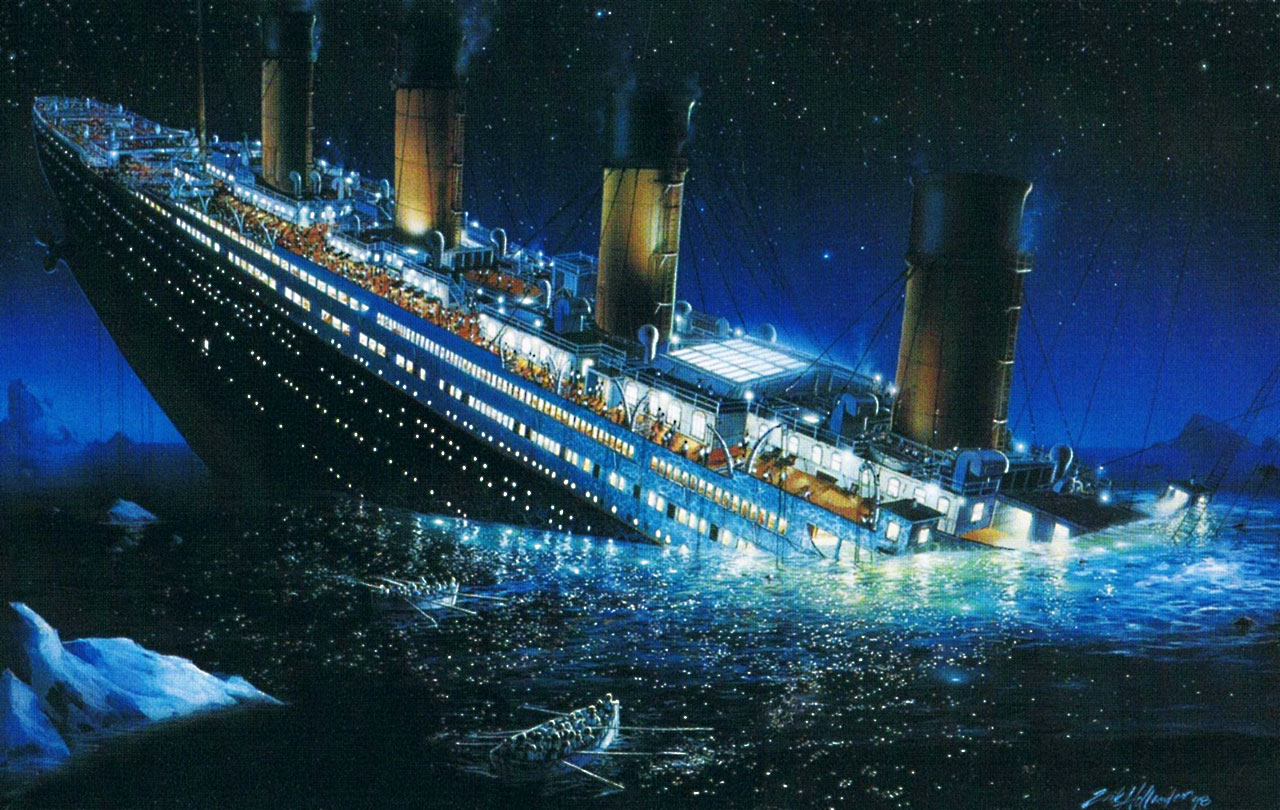
\includegraphics{images/titanic.jpg}
\caption{titanic}
\end{figure}

    \hypertarget{i.-research}{%
\section{I. Research}\label{i.-research}}

\begin{figure}
\centering
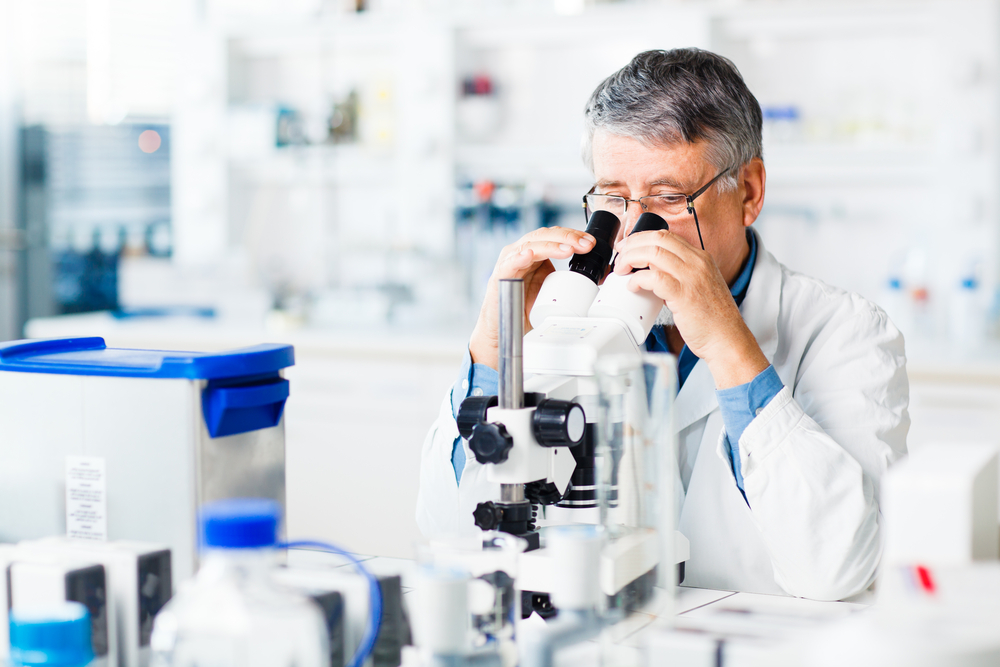
\includegraphics{images/research.jpg}
\caption{research}
\end{figure}

    \hypertarget{ux447ux442ux43e-ux438ux441ux43fux43eux43bux44cux437ux443ux435ux43c}{%
\section{Что
используем?}\label{ux447ux442ux43e-ux438ux441ux43fux43eux43bux44cux437ux443ux435ux43c}}

    \begin{Verbatim}[commandchars=\\\{\}]
{\color{incolor}In [{\color{incolor}17}]:} \PY{k+kn}{import} \PY{n+nn}{warnings}
         \PY{n}{warnings}\PY{o}{.}\PY{n}{filterwarnings}\PY{p}{(}\PY{n}{action}\PY{o}{=}\PY{l+s+s2}{\PYZdq{}}\PY{l+s+s2}{ignore}\PY{l+s+s2}{\PYZdq{}}\PY{p}{,} \PY{n}{module}\PY{o}{=}\PY{l+s+s2}{\PYZdq{}}\PY{l+s+s2}{scipy}\PY{l+s+s2}{\PYZdq{}}\PY{p}{,} \PY{n}{message}\PY{o}{=}\PY{l+s+s2}{\PYZdq{}}\PY{l+s+s2}{\PYZca{}internal gelsd}\PY{l+s+s2}{\PYZdq{}}\PY{p}{)}
         
         \PY{k+kn}{from} \PY{n+nn}{sklearn} \PY{k}{import} \PY{n}{linear\PYZus{}model}
         \PY{k+kn}{from} \PY{n+nn}{sklearn} \PY{k}{import} \PY{n}{preprocessing}
         \PY{k+kn}{from} \PY{n+nn}{sklearn} \PY{k}{import} \PY{n}{metrics}
         \PY{k+kn}{from} \PY{n+nn}{sklearn}\PY{n+nn}{.}\PY{n+nn}{externals} \PY{k}{import} \PY{n}{joblib}
         \PY{k+kn}{from} \PY{n+nn}{sklearn}\PY{n+nn}{.}\PY{n+nn}{model\PYZus{}selection} \PY{k}{import} \PY{n}{train\PYZus{}test\PYZus{}split}
         \PY{k+kn}{import} \PY{n+nn}{pandas} \PY{k}{as} \PY{n+nn}{pd}
         
         \PY{k+kn}{import} \PY{n+nn}{matplotlib}\PY{n+nn}{.}\PY{n+nn}{pyplot} \PY{k}{as} \PY{n+nn}{plt}
\end{Verbatim}


    \hypertarget{ux447ux442ux435ux43dux438ux435-ux434ux430ux43dux43dux44bux445}{%
\subsection{Чтение
данных}\label{ux447ux442ux435ux43dux438ux435-ux434ux430ux43dux43dux44bux445}}

    \begin{Verbatim}[commandchars=\\\{\}]
{\color{incolor}In [{\color{incolor}18}]:} \PY{n}{data} \PY{o}{=} \PY{n}{pd}\PY{o}{.}\PY{n}{read\PYZus{}csv}\PY{p}{(}\PY{l+s+s1}{\PYZsq{}}\PY{l+s+s1}{./data/passengers\PYZus{}info.csv}\PY{l+s+s1}{\PYZsq{}}\PY{p}{)}
\end{Verbatim}


    \begin{Verbatim}[commandchars=\\\{\}]
{\color{incolor}In [{\color{incolor}19}]:} \PY{n}{data}\PY{o}{.}\PY{n}{columns}
\end{Verbatim}


\begin{Verbatim}[commandchars=\\\{\}]
{\color{outcolor}Out[{\color{outcolor}19}]:} Index(['PassengerId', 'Survived', 'Pclass', 'Name', 'Sex', 'Age', 'SibSp',
                'Parch', 'Ticket', 'Fare', 'Cabin', 'Embarked'],
               dtype='object')
\end{Verbatim}
            
    \hypertarget{ux441ux43eux437ux434ux430ux43dux438ux435-baseline}{%
\subsection{Создание
baseline}\label{ux441ux43eux437ux434ux430ux43dux438ux435-baseline}}

\begin{figure}
\centering
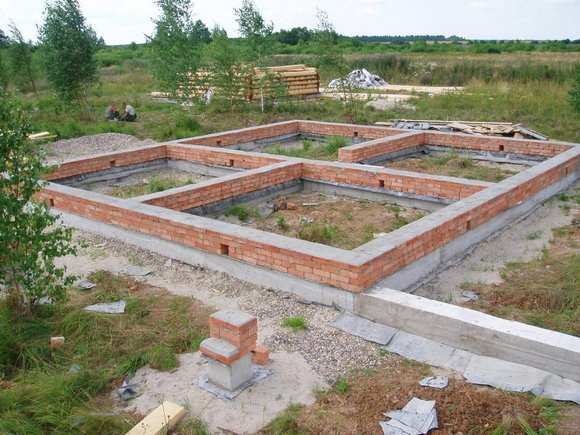
\includegraphics{images/baseline.jpg}
\caption{baseline}
\end{figure}

    \hypertarget{ux441ux43eux437ux434ux430ux43dux438ux435-baseline}{%
\subsection{Создание
baseline}\label{ux441ux43eux437ux434ux430ux43dux438ux435-baseline}}

    \begin{Verbatim}[commandchars=\\\{\}]
{\color{incolor}In [{\color{incolor}20}]:} \PY{n}{features\PYZus{}dataframe} \PY{o}{=} \PY{n}{pd}\PY{o}{.}\PY{n}{DataFrame}\PY{p}{(}\PY{p}{)}
\end{Verbatim}


    \begin{Verbatim}[commandchars=\\\{\}]
{\color{incolor}In [{\color{incolor}21}]:} \PY{n}{array}\PY{p}{,} \PY{n}{levels} \PY{o}{=} \PY{n}{pd}\PY{o}{.}\PY{n}{factorize}\PY{p}{(}\PY{n}{data}\PY{o}{.}\PY{n}{Sex}\PY{p}{)}
         \PY{n}{features\PYZus{}dataframe}\PY{p}{[}\PY{l+s+s1}{\PYZsq{}}\PY{l+s+s1}{factorized\PYZus{}sex}\PY{l+s+s1}{\PYZsq{}}\PY{p}{]} \PY{o}{=} \PY{n}{array}
\end{Verbatim}


    \begin{Verbatim}[commandchars=\\\{\}]
{\color{incolor}In [{\color{incolor}22}]:} \PY{n}{levels}
\end{Verbatim}


\begin{Verbatim}[commandchars=\\\{\}]
{\color{outcolor}Out[{\color{outcolor}22}]:} Index(['male', 'female'], dtype='object')
\end{Verbatim}
            
    \begin{Verbatim}[commandchars=\\\{\}]
{\color{incolor}In [{\color{incolor}23}]:} \PY{n}{features\PYZus{}dataframe}\PY{p}{[}\PY{l+s+s1}{\PYZsq{}}\PY{l+s+s1}{known\PYZus{}age}\PY{l+s+s1}{\PYZsq{}}\PY{p}{]} \PY{o}{=} \PY{n}{data}\PY{o}{.}\PY{n}{Age}\PY{o}{.}\PY{n}{notnull}\PY{p}{(}\PY{p}{)}\PY{o}{.}\PY{n}{astype}\PY{p}{(}\PY{n+nb}{int}\PY{p}{)}
\end{Verbatim}


    \hypertarget{ux43eux431ux443ux447ux430ux44eux449ux438ux435-ux438-ux442ux435ux441ux442ux43eux432ux44bux435-ux432ux44bux431ux43eux440ux43aux438}{%
\subsection{Обучающие и тестовые
выборки}\label{ux43eux431ux443ux447ux430ux44eux449ux438ux435-ux438-ux442ux435ux441ux442ux43eux432ux44bux435-ux432ux44bux431ux43eux440ux43aux438}}

\begin{figure}
\centering
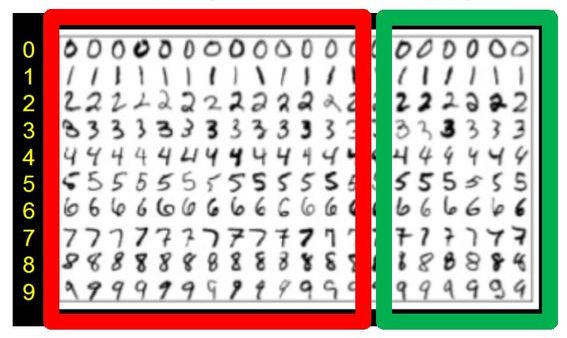
\includegraphics{images/train_test_data.jpg}
\caption{train\_test}
\end{figure}

    \hypertarget{ux43eux431ux443ux447ux430ux44eux449ux438ux435-ux438-ux442ux435ux441ux442ux43eux432ux44bux435-ux432ux44bux431ux43eux440ux43aux438}{%
\subsection{Обучающие и тестовые
выборки}\label{ux43eux431ux443ux447ux430ux44eux449ux438ux435-ux438-ux442ux435ux441ux442ux43eux432ux44bux435-ux432ux44bux431ux43eux440ux43aux438}}

    \begin{Verbatim}[commandchars=\\\{\}]
{\color{incolor}In [{\color{incolor}24}]:} \PY{n}{X} \PY{o}{=} \PY{n}{features\PYZus{}dataframe}
         \PY{n}{y} \PY{o}{=} \PY{n}{data}\PY{o}{.}\PY{n}{Survived}
         \PY{n}{X\PYZus{}train}\PY{p}{,} \PY{n}{X\PYZus{}test}\PY{p}{,} \PY{n}{y\PYZus{}train}\PY{p}{,} \PY{n}{y\PYZus{}test} \PY{o}{=} \PY{n}{train\PYZus{}test\PYZus{}split}\PY{p}{(}\PY{n}{X}\PY{p}{,} \PY{n}{y}\PY{p}{,} \PY{n}{test\PYZus{}size}\PY{o}{=}\PY{l+m+mf}{0.33}\PY{p}{,} \PY{n}{random\PYZus{}state}\PY{o}{=}\PY{l+m+mi}{0}\PY{p}{)}
\end{Verbatim}


    \begin{Verbatim}[commandchars=\\\{\}]
{\color{incolor}In [{\color{incolor}25}]:} \PY{p}{(}\PY{n+nb}{len}\PY{p}{(}\PY{n}{X}\PY{p}{)}\PY{p}{,} \PY{n+nb}{len}\PY{p}{(}\PY{n}{X\PYZus{}train}\PY{p}{)}\PY{p}{,} \PY{n+nb}{len}\PY{p}{(}\PY{n}{X\PYZus{}test}\PY{p}{)}\PY{p}{)}
\end{Verbatim}


\begin{Verbatim}[commandchars=\\\{\}]
{\color{outcolor}Out[{\color{outcolor}25}]:} (891, 596, 295)
\end{Verbatim}
            
    \hypertarget{ux43bux438ux43dux435ux439ux43dux430ux44f-ux440ux435ux433ux440ux435ux441ux441ux438ux44f}{%
\subsection{Линейная
регрессия}\label{ux43bux438ux43dux435ux439ux43dux430ux44f-ux440ux435ux433ux440ux435ux441ux441ux438ux44f}}

\[y = f(\vec{w}\cdot\vec{x}) = f\left(\sum_j w_j x_j\right)\]

\begin{figure}
\centering
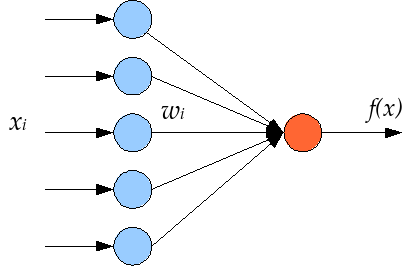
\includegraphics{images/perceptron.png}
\caption{perseptron}
\end{figure}

    \hypertarget{ux43bux438ux43dux435ux439ux43dux430ux44f-ux440ux435ux433ux440ux435ux441ux441ux438ux44f}{%
\subsection{Линейная
регрессия}\label{ux43bux438ux43dux435ux439ux43dux430ux44f-ux440ux435ux433ux440ux435ux441ux441ux438ux44f}}

    \begin{Verbatim}[commandchars=\\\{\}]
{\color{incolor}In [{\color{incolor}26}]:} \PY{n}{reg} \PY{o}{=} \PY{n}{linear\PYZus{}model}\PY{o}{.}\PY{n}{LinearRegression}\PY{p}{(}\PY{p}{)}
         \PY{n}{reg}\PY{o}{.}\PY{n}{fit}\PY{p}{(}\PY{n}{X\PYZus{}train}\PY{p}{,} \PY{n}{y\PYZus{}train}\PY{p}{)}
\end{Verbatim}


\begin{Verbatim}[commandchars=\\\{\}]
{\color{outcolor}Out[{\color{outcolor}26}]:} LinearRegression(copy\_X=True, fit\_intercept=True, n\_jobs=1, normalize=False)
\end{Verbatim}
            
    \hypertarget{ux43eux446ux435ux43dux43aux430-ux440ux435ux437ux443ux43bux44cux442ux430ux442ux430}{%
\section{Оценка
результата}\label{ux43eux446ux435ux43dux43aux430-ux440ux435ux437ux443ux43bux44cux442ux430ux442ux430}}

    \begin{Verbatim}[commandchars=\\\{\}]
{\color{incolor}In [{\color{incolor}27}]:} \PY{n}{y\PYZus{}predicted} \PY{o}{=} \PY{n}{reg}\PY{o}{.}\PY{n}{predict}\PY{p}{(}\PY{n}{X\PYZus{}test}\PY{p}{)}
\end{Verbatim}


    \begin{Verbatim}[commandchars=\\\{\}]
{\color{incolor}In [{\color{incolor}28}]:} \PY{n}{y\PYZus{}predicted}
\end{Verbatim}


\begin{Verbatim}[commandchars=\\\{\}]
{\color{outcolor}Out[{\color{outcolor}28}]:} array([0.12500426, 0.12500426, 0.21166028, 0.68381376, 0.77046978,
                0.12500426, 0.77046978, 0.77046978, 0.21166028, 0.68381376,
                0.21166028, 0.77046978, 0.12500426, 0.77046978, 0.77046978,
                0.77046978, 0.21166028, 0.21166028, 0.21166028, 0.21166028,
                0.21166028, 0.77046978, 0.12500426, 0.12500426, 0.77046978,
                0.77046978, 0.21166028, 0.77046978, 0.77046978, 0.77046978,
                0.21166028, 0.77046978, 0.21166028, 0.12500426, 0.21166028,
                0.21166028, 0.21166028, 0.21166028, 0.21166028, 0.21166028,
                0.21166028, 0.21166028, 0.12500426, 0.21166028, 0.77046978,
                0.12500426, 0.12500426, 0.77046978, 0.21166028, 0.21166028,
                0.12500426, 0.21166028, 0.77046978, 0.21166028, 0.12500426,
                0.21166028, 0.21166028, 0.77046978, 0.21166028, 0.12500426,
                0.21166028, 0.77046978, 0.77046978, 0.12500426, 0.77046978,
                0.21166028, 0.77046978, 0.21166028, 0.77046978, 0.77046978,
                0.77046978, 0.21166028, 0.21166028, 0.12500426, 0.21166028,
                0.77046978, 0.21166028, 0.21166028, 0.21166028, 0.12500426,
                0.12500426, 0.21166028, 0.77046978, 0.21166028, 0.21166028,
                0.77046978, 0.77046978, 0.77046978, 0.77046978, 0.21166028,
                0.12500426, 0.21166028, 0.21166028, 0.77046978, 0.77046978,
                0.12500426, 0.77046978, 0.21166028, 0.21166028, 0.21166028,
                0.21166028, 0.21166028, 0.21166028, 0.21166028, 0.77046978,
                0.77046978, 0.77046978, 0.77046978, 0.21166028, 0.68381376,
                0.21166028, 0.77046978, 0.21166028, 0.68381376, 0.21166028,
                0.77046978, 0.77046978, 0.77046978, 0.21166028, 0.77046978,
                0.12500426, 0.12500426, 0.21166028, 0.21166028, 0.21166028,
                0.21166028, 0.12500426, 0.21166028, 0.12500426, 0.21166028,
                0.77046978, 0.21166028, 0.21166028, 0.77046978, 0.21166028,
                0.21166028, 0.12500426, 0.77046978, 0.21166028, 0.21166028,
                0.21166028, 0.77046978, 0.12500426, 0.77046978, 0.68381376,
                0.77046978, 0.21166028, 0.77046978, 0.77046978, 0.12500426,
                0.21166028, 0.77046978, 0.77046978, 0.21166028, 0.77046978,
                0.21166028, 0.77046978, 0.21166028, 0.68381376, 0.77046978,
                0.12500426, 0.21166028, 0.77046978, 0.77046978, 0.21166028,
                0.21166028, 0.21166028, 0.21166028, 0.21166028, 0.21166028,
                0.21166028, 0.77046978, 0.12500426, 0.12500426, 0.77046978,
                0.12500426, 0.77046978, 0.21166028, 0.21166028, 0.68381376,
                0.21166028, 0.21166028, 0.21166028, 0.21166028, 0.21166028,
                0.21166028, 0.68381376, 0.12500426, 0.21166028, 0.77046978,
                0.77046978, 0.21166028, 0.77046978, 0.68381376, 0.12500426,
                0.21166028, 0.12500426, 0.77046978, 0.21166028, 0.21166028,
                0.21166028, 0.68381376, 0.21166028, 0.77046978, 0.21166028,
                0.21166028, 0.77046978, 0.21166028, 0.77046978, 0.21166028,
                0.21166028, 0.21166028, 0.21166028, 0.77046978, 0.21166028,
                0.21166028, 0.21166028, 0.21166028, 0.77046978, 0.68381376,
                0.21166028, 0.77046978, 0.77046978, 0.21166028, 0.77046978,
                0.21166028, 0.21166028, 0.77046978, 0.21166028, 0.21166028,
                0.21166028, 0.77046978, 0.77046978, 0.77046978, 0.21166028,
                0.21166028, 0.77046978, 0.77046978, 0.77046978, 0.12500426,
                0.12500426, 0.77046978, 0.21166028, 0.21166028, 0.77046978,
                0.12500426, 0.68381376, 0.12500426, 0.12500426, 0.77046978,
                0.21166028, 0.21166028, 0.21166028, 0.12500426, 0.77046978,
                0.77046978, 0.68381376, 0.21166028, 0.21166028, 0.21166028,
                0.12500426, 0.12500426, 0.21166028, 0.21166028, 0.12500426,
                0.21166028, 0.77046978, 0.12500426, 0.21166028, 0.77046978,
                0.21166028, 0.21166028, 0.68381376, 0.21166028, 0.21166028,
                0.21166028, 0.21166028, 0.21166028, 0.68381376, 0.68381376,
                0.21166028, 0.68381376, 0.12500426, 0.77046978, 0.21166028,
                0.21166028, 0.21166028, 0.68381376, 0.21166028, 0.12500426,
                0.12500426, 0.21166028, 0.68381376, 0.77046978, 0.77046978])
\end{Verbatim}
            
    \hypertarget{ux43eux446ux435ux43dux43aux430-ux440ux435ux437ux443ux43bux44cux442ux430ux442ux430}{%
\section{Оценка
результата}\label{ux43eux446ux435ux43dux43aux430-ux440ux435ux437ux443ux43bux44cux442ux430ux442ux430}}

\hypertarget{ux43aux440ux438ux432ux430ux44f-ux43eux448ux438ux431ux43eux43a}{%
\subsection{Кривая
ошибок}\label{ux43aux440ux438ux432ux430ux44f-ux43eux448ux438ux431ux43eux43a}}

\begin{figure}
\centering
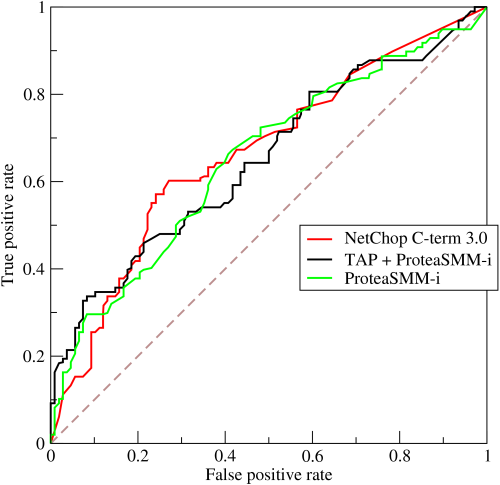
\includegraphics{images/roc_curves.png}
\caption{roc}
\end{figure}

    \hypertarget{ux43eux446ux435ux43dux43aux430-ux440ux435ux437ux443ux43bux44cux442ux430ux442ux430}{%
\section{Оценка
результата}\label{ux43eux446ux435ux43dux43aux430-ux440ux435ux437ux443ux43bux44cux442ux430ux442ux430}}

    \begin{Verbatim}[commandchars=\\\{\}]
{\color{incolor}In [{\color{incolor}29}]:} \PY{n}{fpr}\PY{p}{,} \PY{n}{tpr}\PY{p}{,} \PY{n}{\PYZus{}} \PY{o}{=} \PY{n}{metrics}\PY{o}{.}\PY{n}{roc\PYZus{}curve}\PY{p}{(}\PY{n}{y\PYZus{}test}\PY{p}{,} \PY{n}{y\PYZus{}predicted}\PY{p}{)}
         \PY{n}{roc\PYZus{}auc} \PY{o}{=} \PY{n}{metrics}\PY{o}{.}\PY{n}{auc}\PY{p}{(}\PY{n}{fpr}\PY{p}{,} \PY{n}{tpr}\PY{p}{)}
         
         \PY{k}{def} \PY{n+nf}{init\PYZus{}plt}\PY{p}{(}\PY{p}{)}\PY{p}{:}
             \PY{n}{plt}\PY{o}{.}\PY{n}{figure}\PY{p}{(}\PY{n}{figsize}\PY{o}{=}\PY{p}{(}\PY{l+m+mi}{14}\PY{p}{,}\PY{l+m+mi}{7}\PY{p}{)}\PY{p}{)}
             \PY{n}{lw} \PY{o}{=} \PY{l+m+mi}{2}
             \PY{n}{plt}\PY{o}{.}\PY{n}{plot}\PY{p}{(}\PY{p}{[}\PY{l+m+mi}{0}\PY{p}{,} \PY{l+m+mi}{1}\PY{p}{]}\PY{p}{,} \PY{p}{[}\PY{l+m+mi}{0}\PY{p}{,} \PY{l+m+mi}{1}\PY{p}{]}\PY{p}{,} \PY{n}{color}\PY{o}{=}\PY{l+s+s1}{\PYZsq{}}\PY{l+s+s1}{navy}\PY{l+s+s1}{\PYZsq{}}\PY{p}{,} \PY{n}{lw}\PY{o}{=}\PY{n}{lw}\PY{p}{,} \PY{n}{linestyle}\PY{o}{=}\PY{l+s+s1}{\PYZsq{}}\PY{l+s+s1}{\PYZhy{}\PYZhy{}}\PY{l+s+s1}{\PYZsq{}}\PY{p}{)}
             \PY{n}{plt}\PY{o}{.}\PY{n}{xlim}\PY{p}{(}\PY{p}{[}\PY{l+m+mf}{0.0}\PY{p}{,} \PY{l+m+mf}{1.0}\PY{p}{]}\PY{p}{)}
             \PY{n}{plt}\PY{o}{.}\PY{n}{ylim}\PY{p}{(}\PY{p}{[}\PY{l+m+mf}{0.0}\PY{p}{,} \PY{l+m+mf}{1.05}\PY{p}{]}\PY{p}{)}
             \PY{n}{plt}\PY{o}{.}\PY{n}{xlabel}\PY{p}{(}\PY{l+s+s1}{\PYZsq{}}\PY{l+s+s1}{False Positive Rate}\PY{l+s+s1}{\PYZsq{}}\PY{p}{)}
             \PY{n}{plt}\PY{o}{.}\PY{n}{ylabel}\PY{p}{(}\PY{l+s+s1}{\PYZsq{}}\PY{l+s+s1}{True Positive Rate}\PY{l+s+s1}{\PYZsq{}}\PY{p}{)}
             \PY{n}{plt}\PY{o}{.}\PY{n}{title}\PY{p}{(}\PY{l+s+s1}{\PYZsq{}}\PY{l+s+s1}{Receiver operating characteristic example}\PY{l+s+s1}{\PYZsq{}}\PY{p}{)}
             
         \PY{n}{roc\PYZus{}auc}
\end{Verbatim}


\begin{Verbatim}[commandchars=\\\{\}]
{\color{outcolor}Out[{\color{outcolor}29}]:} 0.7747747747747749
\end{Verbatim}
            
    \hypertarget{ux43eux446ux435ux43dux43aux430-ux440ux435ux437ux443ux43bux44cux442ux430ux442ux430}{%
\section{Оценка
результата}\label{ux43eux446ux435ux43dux43aux430-ux440ux435ux437ux443ux43bux44cux442ux430ux442ux430}}

    \begin{Verbatim}[commandchars=\\\{\}]
{\color{incolor}In [{\color{incolor}30}]:} \PY{n}{init\PYZus{}plt}\PY{p}{(}\PY{p}{)}
         \PY{n}{plt}\PY{o}{.}\PY{n}{plot}\PY{p}{(}\PY{n}{fpr}\PY{p}{,} \PY{n}{tpr}\PY{p}{,} \PY{n}{color}\PY{o}{=}\PY{l+s+s1}{\PYZsq{}}\PY{l+s+s1}{darkorange}\PY{l+s+s1}{\PYZsq{}}\PY{p}{,} \PY{n}{lw}\PY{o}{=}\PY{l+m+mi}{2}\PY{p}{,} \PY{n}{label}\PY{o}{=}\PY{l+s+s1}{\PYZsq{}}\PY{l+s+s1}{ROC curve (area = }\PY{l+s+si}{\PYZpc{}0.4f}\PY{l+s+s1}{)}\PY{l+s+s1}{\PYZsq{}} \PY{o}{\PYZpc{}} \PY{n}{roc\PYZus{}auc}\PY{p}{)}
         \PY{n}{plt}\PY{o}{.}\PY{n}{legend}\PY{p}{(}\PY{n}{loc}\PY{o}{=}\PY{l+s+s2}{\PYZdq{}}\PY{l+s+s2}{lower right}\PY{l+s+s2}{\PYZdq{}}\PY{p}{)}
         \PY{n}{plt}\PY{o}{.}\PY{n}{show}\PY{p}{(}\PY{p}{)}
\end{Verbatim}


    \begin{Verbatim}[commandchars=\\\{\}]

        ---------------------------------------------------------------------------

        NameError                                 Traceback (most recent call last)

        <ipython-input-30-368713ce0cee> in <module>()
          1 init\_plt()
    ----> 2 plt.plot(fpr, tpr, color='darkorange', lw=lw, label='ROC curve (area = \%0.4f)' \% roc\_auc)
          3 plt.legend(loc="lower right")
          4 plt.show()


        NameError: name 'lw' is not defined

    \end{Verbatim}

    \begin{center}
    \adjustimage{max size={0.9\linewidth}{0.9\paperheight}}{output_32_1.png}
    \end{center}
    { \hspace*{\fill} \\}
    
    \hypertarget{feature-engineering-scaling}{%
\section{Feature engineering:
scaling}\label{feature-engineering-scaling}}

    \begin{Verbatim}[commandchars=\\\{\}]
{\color{incolor}In [{\color{incolor}31}]:} \PY{n}{min\PYZus{}max\PYZus{}scaler} \PY{o}{=} \PY{n}{preprocessing}\PY{o}{.}\PY{n}{MinMaxScaler}\PY{p}{(}\PY{p}{)}
         \PY{n}{features\PYZus{}dataframe}\PY{p}{[}\PY{l+s+s1}{\PYZsq{}}\PY{l+s+s1}{scaled\PYZus{}fare}\PY{l+s+s1}{\PYZsq{}}\PY{p}{]} \PY{o}{=} \PY{n}{min\PYZus{}max\PYZus{}scaler}\PY{o}{.}\PY{n}{fit\PYZus{}transform}\PY{p}{(}\PY{n}{data}\PY{p}{[}\PY{p}{[}\PY{l+s+s1}{\PYZsq{}}\PY{l+s+s1}{Fare}\PY{l+s+s1}{\PYZsq{}}\PY{p}{]}\PY{p}{]}\PY{p}{)}
\end{Verbatim}


    \begin{Verbatim}[commandchars=\\\{\}]
{\color{incolor}In [{\color{incolor}32}]:} \PY{n}{features\PYZus{}dataframe}
\end{Verbatim}


\begin{Verbatim}[commandchars=\\\{\}]
{\color{outcolor}Out[{\color{outcolor}32}]:}      factorized\_sex  known\_age  scaled\_fare
         0                 0          1     0.014151
         1                 1          1     0.139136
         2                 1          1     0.015469
         3                 1          1     0.103644
         4                 0          1     0.015713
         5                 0          0     0.016510
         6                 0          1     0.101229
         7                 0          1     0.041136
         8                 1          1     0.021731
         9                 1          1     0.058694
         10                1          1     0.032596
         11                1          1     0.051822
         12                0          1     0.015713
         13                0          1     0.061045
         14                1          1     0.015330
         15                1          1     0.031230
         16                0          1     0.056848
         17                0          0     0.025374
         18                1          1     0.035134
         19                1          0     0.014102
         20                0          1     0.050749
         21                0          1     0.025374
         22                1          1     0.015672
         23                0          1     0.069291
         24                1          1     0.041136
         25                1          1     0.061264
         26                0          0     0.014102
         27                0          1     0.513342
         28                1          0     0.015379
         29                0          0     0.015412
         ..              {\ldots}        {\ldots}          {\ldots}
         861               0          1     0.022447
         862               1          1     0.050610
         863               1          0     0.135753
         864               0          1     0.025374
         865               1          1     0.025374
         866               1          1     0.027050
         867               0          1     0.098561
         868               0          0     0.018543
         869               0          1     0.021731
         870               0          1     0.015412
         871               1          1     0.102579
         872               0          1     0.009759
         873               0          1     0.017567
         874               1          1     0.046845
         875               1          1     0.014102
         876               0          1     0.019218
         877               0          1     0.015412
         878               0          0     0.015412
         879               1          1     0.162314
         880               1          1     0.050749
         881               0          1     0.015412
         882               1          1     0.020527
         883               0          1     0.020495
         884               0          1     0.013761
         885               1          1     0.056848
         886               0          1     0.025374
         887               1          1     0.058556
         888               1          0     0.045771
         889               0          1     0.058556
         890               0          1     0.015127
         
         [891 rows x 3 columns]
\end{Verbatim}
            
    \hypertarget{feature-engineering-ux43aux430ux442ux435ux433ux43eux440ux438ux430ux43bux44cux43dux44bux435-ux43fux440ux438ux437ux43dux430ux43aux438}{%
\section{Feature engineering: категориальные
признаки}\label{feature-engineering-ux43aux430ux442ux435ux433ux43eux440ux438ux430ux43bux44cux43dux44bux435-ux43fux440ux438ux437ux43dux430ux43aux438}}

    \begin{Verbatim}[commandchars=\\\{\}]
{\color{incolor}In [{\color{incolor}33}]:} \PY{k}{for} \PY{n}{cl\PYZus{}num} \PY{o+ow}{in} \PY{p}{[}\PY{l+m+mi}{1}\PY{p}{,} \PY{l+m+mi}{2}\PY{p}{]}\PY{p}{:}
             \PY{n}{name} \PY{o}{=} \PY{l+s+s1}{\PYZsq{}}\PY{l+s+s1}{class}\PY{l+s+si}{\PYZob{}\PYZcb{}}\PY{l+s+s1}{\PYZsq{}}\PY{o}{.}\PY{n}{format}\PY{p}{(}\PY{n}{cl\PYZus{}num}\PY{p}{)}
             \PY{n}{features\PYZus{}dataframe}\PY{p}{[}\PY{n}{name}\PY{p}{]} \PY{o}{=} \PY{p}{(}\PY{n}{data}\PY{p}{[}\PY{l+s+s1}{\PYZsq{}}\PY{l+s+s1}{Pclass}\PY{l+s+s1}{\PYZsq{}}\PY{p}{]} \PY{o}{==} \PY{n}{cl\PYZus{}num}\PY{p}{)}\PY{o}{.}\PY{n}{astype}\PY{p}{(}\PY{n+nb}{int}\PY{p}{)}
         
         \PY{k}{for} \PY{n}{sp} \PY{o+ow}{in} \PY{p}{[}\PY{l+m+mi}{1}\PY{p}{,} \PY{l+m+mi}{2}\PY{p}{,} \PY{l+m+mi}{3}\PY{p}{,} \PY{l+m+mi}{4}\PY{p}{]}\PY{p}{:}
             \PY{n}{name} \PY{o}{=} \PY{l+s+s1}{\PYZsq{}}\PY{l+s+s1}{sib\PYZus{}sp\PYZus{}}\PY{l+s+si}{\PYZob{}\PYZcb{}}\PY{l+s+s1}{\PYZsq{}}\PY{o}{.}\PY{n}{format}\PY{p}{(}\PY{n}{sp}\PY{p}{)}
             \PY{n}{features\PYZus{}dataframe}\PY{p}{[}\PY{n}{name}\PY{p}{]} \PY{o}{=} \PY{p}{(}\PY{n}{data}\PY{o}{.}\PY{n}{SibSp} \PY{o}{==} \PY{n}{sp}\PY{p}{)}\PY{o}{.}\PY{n}{astype}\PY{p}{(}\PY{n+nb}{int}\PY{p}{)}
             
         \PY{k}{for} \PY{n}{emb} \PY{o+ow}{in} \PY{p}{[}\PY{l+s+s1}{\PYZsq{}}\PY{l+s+s1}{C}\PY{l+s+s1}{\PYZsq{}}\PY{p}{,} \PY{l+s+s1}{\PYZsq{}}\PY{l+s+s1}{Q}\PY{l+s+s1}{\PYZsq{}}\PY{p}{,} \PY{l+s+s1}{\PYZsq{}}\PY{l+s+s1}{S}\PY{l+s+s1}{\PYZsq{}}\PY{p}{]}\PY{p}{:}
             \PY{n}{name} \PY{o}{=} \PY{l+s+s1}{\PYZsq{}}\PY{l+s+s1}{embarked}\PY{l+s+si}{\PYZob{}\PYZcb{}}\PY{l+s+s1}{\PYZsq{}}\PY{o}{.}\PY{n}{format}\PY{p}{(}\PY{n}{emb}\PY{p}{)}
             \PY{n}{features\PYZus{}dataframe}\PY{p}{[}\PY{n}{name}\PY{p}{]} \PY{o}{=} \PY{p}{(}\PY{n}{data}\PY{o}{.}\PY{n}{Embarked} \PY{o}{==} \PY{n}{emb}\PY{p}{)}\PY{o}{.}\PY{n}{astype}\PY{p}{(}\PY{n+nb}{int}\PY{p}{)} 
             
         \PY{k}{for} \PY{n}{age} \PY{o+ow}{in} \PY{p}{[}\PY{l+m+mi}{10}\PY{p}{,} \PY{l+m+mi}{20}\PY{p}{,} \PY{l+m+mi}{30}\PY{p}{,} \PY{l+m+mi}{40}\PY{p}{,} \PY{l+m+mi}{50}\PY{p}{,} \PY{l+m+mi}{60}\PY{p}{,} \PY{l+m+mi}{70}\PY{p}{]}\PY{p}{:}
             \PY{n}{name} \PY{o}{=} \PY{l+s+s1}{\PYZsq{}}\PY{l+s+s1}{more\PYZus{}}\PY{l+s+si}{\PYZob{}\PYZcb{}}\PY{l+s+s1}{\PYZus{}years}\PY{l+s+s1}{\PYZsq{}}\PY{o}{.}\PY{n}{format}\PY{p}{(}\PY{n}{age}\PY{p}{)}
             \PY{n}{features\PYZus{}dataframe}\PY{p}{[}\PY{n}{name}\PY{p}{]} \PY{o}{=} \PY{p}{(}\PY{n}{data}\PY{p}{[}\PY{l+s+s1}{\PYZsq{}}\PY{l+s+s1}{Age}\PY{l+s+s1}{\PYZsq{}}\PY{p}{]} \PY{o}{\PYZgt{}}\PY{o}{=} \PY{n}{age}\PY{p}{)}\PY{o}{.}\PY{n}{astype}\PY{p}{(}\PY{n+nb}{int}\PY{p}{)}
\end{Verbatim}


    \begin{Verbatim}[commandchars=\\\{\}]
{\color{incolor}In [{\color{incolor}34}]:} \PY{n}{features\PYZus{}dataframe}
\end{Verbatim}


\begin{Verbatim}[commandchars=\\\{\}]
{\color{outcolor}Out[{\color{outcolor}34}]:}      factorized\_sex  known\_age  scaled\_fare  class1  class2  sib\_sp\_1  \textbackslash{}
         0                 0          1     0.014151       0       0         1   
         1                 1          1     0.139136       1       0         1   
         2                 1          1     0.015469       0       0         0   
         3                 1          1     0.103644       1       0         1   
         4                 0          1     0.015713       0       0         0   
         5                 0          0     0.016510       0       0         0   
         6                 0          1     0.101229       1       0         0   
         7                 0          1     0.041136       0       0         0   
         8                 1          1     0.021731       0       0         0   
         9                 1          1     0.058694       0       1         1   
         10                1          1     0.032596       0       0         1   
         11                1          1     0.051822       1       0         0   
         12                0          1     0.015713       0       0         0   
         13                0          1     0.061045       0       0         1   
         14                1          1     0.015330       0       0         0   
         15                1          1     0.031230       0       1         0   
         16                0          1     0.056848       0       0         0   
         17                0          0     0.025374       0       1         0   
         18                1          1     0.035134       0       0         1   
         19                1          0     0.014102       0       0         0   
         20                0          1     0.050749       0       1         0   
         21                0          1     0.025374       0       1         0   
         22                1          1     0.015672       0       0         0   
         23                0          1     0.069291       1       0         0   
         24                1          1     0.041136       0       0         0   
         25                1          1     0.061264       0       0         1   
         26                0          0     0.014102       0       0         0   
         27                0          1     0.513342       1       0         0   
         28                1          0     0.015379       0       0         0   
         29                0          0     0.015412       0       0         0   
         ..              {\ldots}        {\ldots}          {\ldots}     {\ldots}     {\ldots}       {\ldots}   
         861               0          1     0.022447       0       1         1   
         862               1          1     0.050610       1       0         0   
         863               1          0     0.135753       0       0         0   
         864               0          1     0.025374       0       1         0   
         865               1          1     0.025374       0       1         0   
         866               1          1     0.027050       0       1         1   
         867               0          1     0.098561       1       0         0   
         868               0          0     0.018543       0       0         0   
         869               0          1     0.021731       0       0         1   
         870               0          1     0.015412       0       0         0   
         871               1          1     0.102579       1       0         1   
         872               0          1     0.009759       1       0         0   
         873               0          1     0.017567       0       0         0   
         874               1          1     0.046845       0       1         1   
         875               1          1     0.014102       0       0         0   
         876               0          1     0.019218       0       0         0   
         877               0          1     0.015412       0       0         0   
         878               0          0     0.015412       0       0         0   
         879               1          1     0.162314       1       0         0   
         880               1          1     0.050749       0       1         0   
         881               0          1     0.015412       0       0         0   
         882               1          1     0.020527       0       0         0   
         883               0          1     0.020495       0       1         0   
         884               0          1     0.013761       0       0         0   
         885               1          1     0.056848       0       0         0   
         886               0          1     0.025374       0       1         0   
         887               1          1     0.058556       1       0         0   
         888               1          0     0.045771       0       0         1   
         889               0          1     0.058556       1       0         0   
         890               0          1     0.015127       0       0         0   
         
              sib\_sp\_2  sib\_sp\_3  sib\_sp\_4  embarkedC  embarkedQ  embarkedS  \textbackslash{}
         0           0         0         0          0          0          1   
         1           0         0         0          1          0          0   
         2           0         0         0          0          0          1   
         3           0         0         0          0          0          1   
         4           0         0         0          0          0          1   
         5           0         0         0          0          1          0   
         6           0         0         0          0          0          1   
         7           0         1         0          0          0          1   
         8           0         0         0          0          0          1   
         9           0         0         0          1          0          0   
         10          0         0         0          0          0          1   
         11          0         0         0          0          0          1   
         12          0         0         0          0          0          1   
         13          0         0         0          0          0          1   
         14          0         0         0          0          0          1   
         15          0         0         0          0          0          1   
         16          0         0         1          0          1          0   
         17          0         0         0          0          0          1   
         18          0         0         0          0          0          1   
         19          0         0         0          1          0          0   
         20          0         0         0          0          0          1   
         21          0         0         0          0          0          1   
         22          0         0         0          0          1          0   
         23          0         0         0          0          0          1   
         24          0         1         0          0          0          1   
         25          0         0         0          0          0          1   
         26          0         0         0          1          0          0   
         27          0         1         0          0          0          1   
         28          0         0         0          0          1          0   
         29          0         0         0          0          0          1   
         ..        {\ldots}       {\ldots}       {\ldots}        {\ldots}        {\ldots}        {\ldots}   
         861         0         0         0          0          0          1   
         862         0         0         0          0          0          1   
         863         0         0         0          0          0          1   
         864         0         0         0          0          0          1   
         865         0         0         0          0          0          1   
         866         0         0         0          1          0          0   
         867         0         0         0          0          0          1   
         868         0         0         0          0          0          1   
         869         0         0         0          0          0          1   
         870         0         0         0          0          0          1   
         871         0         0         0          0          0          1   
         872         0         0         0          0          0          1   
         873         0         0         0          0          0          1   
         874         0         0         0          1          0          0   
         875         0         0         0          1          0          0   
         876         0         0         0          0          0          1   
         877         0         0         0          0          0          1   
         878         0         0         0          0          0          1   
         879         0         0         0          1          0          0   
         880         0         0         0          0          0          1   
         881         0         0         0          0          0          1   
         882         0         0         0          0          0          1   
         883         0         0         0          0          0          1   
         884         0         0         0          0          0          1   
         885         0         0         0          0          1          0   
         886         0         0         0          0          0          1   
         887         0         0         0          0          0          1   
         888         0         0         0          0          0          1   
         889         0         0         0          1          0          0   
         890         0         0         0          0          1          0   
         
              more\_10\_years  more\_20\_years  more\_30\_years  more\_40\_years  \textbackslash{}
         0                1              1              0              0   
         1                1              1              1              0   
         2                1              1              0              0   
         3                1              1              1              0   
         4                1              1              1              0   
         5                0              0              0              0   
         6                1              1              1              1   
         7                0              0              0              0   
         8                1              1              0              0   
         9                1              0              0              0   
         10               0              0              0              0   
         11               1              1              1              1   
         12               1              1              0              0   
         13               1              1              1              0   
         14               1              0              0              0   
         15               1              1              1              1   
         16               0              0              0              0   
         17               0              0              0              0   
         18               1              1              1              0   
         19               0              0              0              0   
         20               1              1              1              0   
         21               1              1              1              0   
         22               1              0              0              0   
         23               1              1              0              0   
         24               0              0              0              0   
         25               1              1              1              0   
         26               0              0              0              0   
         27               1              0              0              0   
         28               0              0              0              0   
         29               0              0              0              0   
         ..             {\ldots}            {\ldots}            {\ldots}            {\ldots}   
         861              1              1              0              0   
         862              1              1              1              1   
         863              0              0              0              0   
         864              1              1              0              0   
         865              1              1              1              1   
         866              1              1              0              0   
         867              1              1              1              0   
         868              0              0              0              0   
         869              0              0              0              0   
         870              1              1              0              0   
         871              1              1              1              1   
         872              1              1              1              0   
         873              1              1              1              1   
         874              1              1              0              0   
         875              1              0              0              0   
         876              1              1              0              0   
         877              1              0              0              0   
         878              0              0              0              0   
         879              1              1              1              1   
         880              1              1              0              0   
         881              1              1              1              0   
         882              1              1              0              0   
         883              1              1              0              0   
         884              1              1              0              0   
         885              1              1              1              0   
         886              1              1              0              0   
         887              1              0              0              0   
         888              0              0              0              0   
         889              1              1              0              0   
         890              1              1              1              0   
         
              more\_50\_years  more\_60\_years  more\_70\_years  
         0                0              0              0  
         1                0              0              0  
         2                0              0              0  
         3                0              0              0  
         4                0              0              0  
         5                0              0              0  
         6                1              0              0  
         7                0              0              0  
         8                0              0              0  
         9                0              0              0  
         10               0              0              0  
         11               1              0              0  
         12               0              0              0  
         13               0              0              0  
         14               0              0              0  
         15               1              0              0  
         16               0              0              0  
         17               0              0              0  
         18               0              0              0  
         19               0              0              0  
         20               0              0              0  
         21               0              0              0  
         22               0              0              0  
         23               0              0              0  
         24               0              0              0  
         25               0              0              0  
         26               0              0              0  
         27               0              0              0  
         28               0              0              0  
         29               0              0              0  
         ..             {\ldots}            {\ldots}            {\ldots}  
         861              0              0              0  
         862              0              0              0  
         863              0              0              0  
         864              0              0              0  
         865              0              0              0  
         866              0              0              0  
         867              0              0              0  
         868              0              0              0  
         869              0              0              0  
         870              0              0              0  
         871              0              0              0  
         872              0              0              0  
         873              0              0              0  
         874              0              0              0  
         875              0              0              0  
         876              0              0              0  
         877              0              0              0  
         878              0              0              0  
         879              1              0              0  
         880              0              0              0  
         881              0              0              0  
         882              0              0              0  
         883              0              0              0  
         884              0              0              0  
         885              0              0              0  
         886              0              0              0  
         887              0              0              0  
         888              0              0              0  
         889              0              0              0  
         890              0              0              0  
         
         [891 rows x 19 columns]
\end{Verbatim}
            
    \hypertarget{ux43fux43eux432ux442ux43eux440ux44fux435ux43c-ux43dux430-ux431ux43eux43bux44cux448ux435ux43c-ux447ux438ux441ux43bux435-ux43fux440ux438ux437ux43dux430ux43aux43eux432}{%
\section{Повторяем на большем числе
признаков}\label{ux43fux43eux432ux442ux43eux440ux44fux435ux43c-ux43dux430-ux431ux43eux43bux44cux448ux435ux43c-ux447ux438ux441ux43bux435-ux43fux440ux438ux437ux43dux430ux43aux43eux432}}

    \begin{Verbatim}[commandchars=\\\{\}]
{\color{incolor}In [{\color{incolor}35}]:} \PY{n}{X} \PY{o}{=} \PY{n}{features\PYZus{}dataframe}
         \PY{n}{y} \PY{o}{=} \PY{n}{data}\PY{o}{.}\PY{n}{Survived}
         \PY{n}{X\PYZus{}train}\PY{p}{,} \PY{n}{X\PYZus{}test}\PY{p}{,} \PY{n}{y\PYZus{}train}\PY{p}{,} \PY{n}{y\PYZus{}test} \PY{o}{=} \PY{n}{train\PYZus{}test\PYZus{}split}\PY{p}{(}\PY{n}{X}\PY{p}{,} \PY{n}{y}\PY{p}{,} \PY{n}{test\PYZus{}size}\PY{o}{=}\PY{l+m+mf}{0.33}\PY{p}{,} \PY{n}{random\PYZus{}state}\PY{o}{=}\PY{l+m+mi}{0}\PY{p}{)}
\end{Verbatim}


    \begin{Verbatim}[commandchars=\\\{\}]
{\color{incolor}In [{\color{incolor}36}]:} \PY{n}{reg} \PY{o}{=} \PY{n}{linear\PYZus{}model}\PY{o}{.}\PY{n}{LinearRegression}\PY{p}{(}\PY{p}{)}
         \PY{n}{reg}\PY{o}{.}\PY{n}{fit}\PY{p}{(}\PY{n}{X\PYZus{}train}\PY{p}{,} \PY{n}{y\PYZus{}train}\PY{p}{)}
\end{Verbatim}


\begin{Verbatim}[commandchars=\\\{\}]
{\color{outcolor}Out[{\color{outcolor}36}]:} LinearRegression(copy\_X=True, fit\_intercept=True, n\_jobs=1, normalize=False)
\end{Verbatim}
            
    \begin{Verbatim}[commandchars=\\\{\}]
{\color{incolor}In [{\color{incolor}37}]:} \PY{n}{y\PYZus{}predicted} \PY{o}{=} \PY{n}{reg}\PY{o}{.}\PY{n}{predict}\PY{p}{(}\PY{n}{X\PYZus{}test}\PY{p}{)}
\end{Verbatim}


    \begin{Verbatim}[commandchars=\\\{\}]
{\color{incolor}In [{\color{incolor}38}]:} \PY{n}{fpr\PYZus{}full}\PY{p}{,} \PY{n}{tpr\PYZus{}full}\PY{p}{,} \PY{n}{\PYZus{}} \PY{o}{=} \PY{n}{metrics}\PY{o}{.}\PY{n}{roc\PYZus{}curve}\PY{p}{(}\PY{n}{y\PYZus{}test}\PY{p}{,} \PY{n}{y\PYZus{}predicted}\PY{p}{)}
         \PY{n}{roc\PYZus{}auc\PYZus{}full} \PY{o}{=} \PY{n}{metrics}\PY{o}{.}\PY{n}{auc}\PY{p}{(}\PY{n}{fpr\PYZus{}full}\PY{p}{,} \PY{n}{tpr\PYZus{}full}\PY{p}{)}
         \PY{n}{roc\PYZus{}auc\PYZus{}full}
\end{Verbatim}


    \begin{Verbatim}[commandchars=\\\{\}]
{\color{incolor}In [{\color{incolor}41}]:} \PY{n}{init\PYZus{}plt}\PY{p}{(}\PY{p}{)}
         \PY{n}{plt}\PY{o}{.}\PY{n}{plot}\PY{p}{(}\PY{n}{fpr}\PY{p}{,} \PY{n}{tpr}\PY{p}{,} \PY{n}{color}\PY{o}{=}\PY{l+s+s1}{\PYZsq{}}\PY{l+s+s1}{darkorange}\PY{l+s+s1}{\PYZsq{}}\PY{p}{,} \PY{n}{lw}\PY{o}{=}\PY{l+m+mi}{2}\PY{p}{,} \PY{n}{label}\PY{o}{=}\PY{l+s+s1}{\PYZsq{}}\PY{l+s+s1}{ROC curve (area = }\PY{l+s+si}{\PYZpc{}0.4f}\PY{l+s+s1}{)}\PY{l+s+s1}{\PYZsq{}} \PY{o}{\PYZpc{}} \PY{n}{roc\PYZus{}auc}\PY{p}{)}
         \PY{n}{plt}\PY{o}{.}\PY{n}{plot}\PY{p}{(}\PY{n}{fpr\PYZus{}full}\PY{p}{,} \PY{n}{tpr\PYZus{}full}\PY{p}{,} \PY{n}{color}\PY{o}{=}\PY{l+s+s1}{\PYZsq{}}\PY{l+s+s1}{red}\PY{l+s+s1}{\PYZsq{}}\PY{p}{,} \PY{n}{lw}\PY{o}{=}\PY{l+m+mi}{2}\PY{p}{,} \PY{n}{label}\PY{o}{=}\PY{l+s+s1}{\PYZsq{}}\PY{l+s+s1}{ROC curve (area = }\PY{l+s+si}{\PYZpc{}0.4f}\PY{l+s+s1}{)}\PY{l+s+s1}{\PYZsq{}} \PY{o}{\PYZpc{}} \PY{n}{roc\PYZus{}auc\PYZus{}full}\PY{p}{)}
         \PY{n}{plt}\PY{o}{.}\PY{n}{legend}\PY{p}{(}\PY{n}{loc}\PY{o}{=}\PY{l+s+s2}{\PYZdq{}}\PY{l+s+s2}{lower right}\PY{l+s+s2}{\PYZdq{}}\PY{p}{)}
         \PY{n}{plt}\PY{o}{.}\PY{n}{show}\PY{p}{(}\PY{p}{)}
\end{Verbatim}


    \begin{center}
    \adjustimage{max size={0.9\linewidth}{0.9\paperheight}}{output_44_0.png}
    \end{center}
    { \hspace*{\fill} \\}
    
    \hypertarget{ux431ux43eux43bux44cux448ux435-ux43dux435-ux437ux43dux430ux447ux438ux442-ux43bux443ux447ux448ux435}{%
\section{Больше не значит
лучше}\label{ux431ux43eux43bux44cux448ux435-ux43dux435-ux437ux43dux430ux447ux438ux442-ux43bux443ux447ux448ux435}}

    \begin{Verbatim}[commandchars=\\\{\}]
{\color{incolor}In [{\color{incolor}42}]:} \PY{n}{sorted\PYZus{}features} \PY{o}{=} \PY{n+nb}{list}\PY{p}{(}\PY{n+nb}{sorted}\PY{p}{(}\PY{n+nb}{zip}\PY{p}{(}\PY{n}{features\PYZus{}dataframe}\PY{o}{.}\PY{n}{columns}\PY{p}{,} \PY{n}{reg}\PY{o}{.}\PY{n}{coef\PYZus{}}\PY{p}{)}\PY{p}{,} \PY{n}{key}\PY{o}{=}\PY{k}{lambda} \PY{n}{x}\PY{p}{:} \PY{o}{\PYZhy{}}\PY{n+nb}{abs}\PY{p}{(}\PY{n}{x}\PY{p}{[}\PY{l+m+mi}{1}\PY{p}{]}\PY{p}{)}\PY{p}{)}\PY{p}{)}
         \PY{n}{sorted\PYZus{}features}
\end{Verbatim}


\begin{Verbatim}[commandchars=\\\{\}]
{\color{outcolor}Out[{\color{outcolor}42}]:} [('sib\_sp\_4', -0.5839866903642109),
          ('factorized\_sex', 0.4878065218356281),
          ('sib\_sp\_3', -0.43012605010101934),
          ('known\_age', 0.4163329006803484),
          ('more\_10\_years', -0.36861592370314944),
          ('class1', 0.30573229445465583),
          ('embarkedS', -0.21598195010151952),
          ('class2', 0.15169969725676358),
          ('scaled\_fare', 0.1509233932306982),
          ('embarkedC', -0.12944031947896611),
          ('more\_60\_years', -0.12075027705369325),
          ('embarkedQ', -0.09875948287971013),
          ('sib\_sp\_2', -0.08468604202023416),
          ('more\_40\_years', -0.08250647102947699),
          ('more\_50\_years', -0.057838642959210165),
          ('more\_70\_years', 0.04279030131631274),
          ('sib\_sp\_1', 0.03282222545379855),
          ('more\_20\_years', 0.005178388443575668),
          ('more\_30\_years', 0.0048529582883881095)]
\end{Verbatim}
            
    \hypertarget{ux43fux435ux440ux435ux441ux43cux430ux442ux440ux438ux432ux430ux435ux43c-ux43cux43eux434ux435ux43bux44c-ux43dux430-8-ux43cux438-ux43fux440ux438ux437ux43dux430ux43aux430ux445}{%
\section{Пересматриваем модель на 8-ми
признаках}\label{ux43fux435ux440ux435ux441ux43cux430ux442ux440ux438ux432ux430ux435ux43c-ux43cux43eux434ux435ux43bux44c-ux43dux430-8-ux43cux438-ux43fux440ux438ux437ux43dux430ux43aux430ux445}}

    \begin{Verbatim}[commandchars=\\\{\}]
{\color{incolor}In [{\color{incolor}43}]:} \PY{n}{features\PYZus{}part} \PY{o}{=} \PY{n+nb}{list}\PY{p}{(}\PY{n+nb}{map}\PY{p}{(}\PY{k}{lambda} \PY{n}{x}\PY{p}{:} \PY{n}{x}\PY{p}{[}\PY{l+m+mi}{0}\PY{p}{]}\PY{p}{,} \PY{n}{sorted\PYZus{}features}\PY{p}{[}\PY{p}{:}\PY{l+m+mi}{8}\PY{p}{]}\PY{p}{)}\PY{p}{)}
         \PY{n}{features\PYZus{}part}
\end{Verbatim}


\begin{Verbatim}[commandchars=\\\{\}]
{\color{outcolor}Out[{\color{outcolor}43}]:} ['sib\_sp\_4',
          'factorized\_sex',
          'sib\_sp\_3',
          'known\_age',
          'more\_10\_years',
          'class1',
          'embarkedS',
          'class2']
\end{Verbatim}
            
    \begin{Verbatim}[commandchars=\\\{\}]
{\color{incolor}In [{\color{incolor}44}]:} \PY{n}{X} \PY{o}{=} \PY{n}{features\PYZus{}dataframe}\PY{p}{[}\PY{n}{features\PYZus{}part}\PY{p}{]}
         \PY{n}{y} \PY{o}{=} \PY{n}{data}\PY{o}{.}\PY{n}{Survived}
         \PY{n}{X\PYZus{}train}\PY{p}{,} \PY{n}{X\PYZus{}test}\PY{p}{,} \PY{n}{y\PYZus{}train}\PY{p}{,} \PY{n}{y\PYZus{}test} \PY{o}{=} \PY{n}{train\PYZus{}test\PYZus{}split}\PY{p}{(}\PY{n}{X}\PY{p}{,} \PY{n}{y}\PY{p}{,} \PY{n}{test\PYZus{}size}\PY{o}{=}\PY{l+m+mf}{0.33}\PY{p}{,} \PY{n}{random\PYZus{}state}\PY{o}{=}\PY{l+m+mi}{0}\PY{p}{)}
\end{Verbatim}


    \begin{Verbatim}[commandchars=\\\{\}]
{\color{incolor}In [{\color{incolor}45}]:} \PY{n}{reg} \PY{o}{=} \PY{n}{linear\PYZus{}model}\PY{o}{.}\PY{n}{LinearRegression}\PY{p}{(}\PY{p}{)}
         \PY{n}{reg}\PY{o}{.}\PY{n}{fit}\PY{p}{(}\PY{n}{X\PYZus{}train}\PY{p}{,} \PY{n}{y\PYZus{}train}\PY{p}{)}
         
         \PY{n}{reg}\PY{o}{.}\PY{n}{coef\PYZus{}}
\end{Verbatim}


\begin{Verbatim}[commandchars=\\\{\}]
{\color{outcolor}Out[{\color{outcolor}45}]:} array([-0.57285094,  0.50363661, -0.41594734,  0.40159077, -0.37529241,
                 0.29374776, -0.09615099,  0.14606983])
\end{Verbatim}
            
    \hypertarget{ux43fux435ux440ux435ux441ux43cux430ux442ux440ux438ux432ux430ux435ux43c-ux43cux43eux434ux435ux43bux44c-ux43dux430-8-ux43cux438-ux43fux440ux438ux437ux43dux430ux43aux430ux445}{%
\section{Пересматриваем модель на 8-ми
признаках}\label{ux43fux435ux440ux435ux441ux43cux430ux442ux440ux438ux432ux430ux435ux43c-ux43cux43eux434ux435ux43bux44c-ux43dux430-8-ux43cux438-ux43fux440ux438ux437ux43dux430ux43aux430ux445}}

    \begin{Verbatim}[commandchars=\\\{\}]
{\color{incolor}In [{\color{incolor}46}]:} \PY{n}{y\PYZus{}predicted} \PY{o}{=} \PY{n}{reg}\PY{o}{.}\PY{n}{predict}\PY{p}{(}\PY{n}{X\PYZus{}test}\PY{p}{)}
\end{Verbatim}


    \begin{Verbatim}[commandchars=\\\{\}]
{\color{incolor}In [{\color{incolor}47}]:} \PY{n}{fpr\PYZus{}part}\PY{p}{,} \PY{n}{tpr\PYZus{}part}\PY{p}{,} \PY{n}{thresholds} \PY{o}{=} \PY{n}{metrics}\PY{o}{.}\PY{n}{roc\PYZus{}curve}\PY{p}{(}\PY{n}{y\PYZus{}test}\PY{p}{,} \PY{n}{y\PYZus{}predicted}\PY{p}{)}
         \PY{n}{roc\PYZus{}auc\PYZus{}part} \PY{o}{=} \PY{n}{metrics}\PY{o}{.}\PY{n}{auc}\PY{p}{(}\PY{n}{fpr\PYZus{}part}\PY{p}{,} \PY{n}{tpr\PYZus{}part}\PY{p}{)}
         \PY{n}{roc\PYZus{}auc\PYZus{}part}
\end{Verbatim}


    \begin{Verbatim}[commandchars=\\\{\}]
{\color{incolor}In [{\color{incolor}50}]:} \PY{n}{init\PYZus{}plt}\PY{p}{(}\PY{p}{)}
         \PY{n}{plt}\PY{o}{.}\PY{n}{plot}\PY{p}{(}\PY{n}{fpr}\PY{p}{,} \PY{n}{tpr}\PY{p}{,} \PY{n}{color}\PY{o}{=}\PY{l+s+s1}{\PYZsq{}}\PY{l+s+s1}{darkorange}\PY{l+s+s1}{\PYZsq{}}\PY{p}{,} \PY{n}{lw}\PY{o}{=}\PY{l+m+mi}{2}\PY{p}{,} \PY{n}{label}\PY{o}{=}\PY{l+s+s1}{\PYZsq{}}\PY{l+s+s1}{ROC curve (area = }\PY{l+s+si}{\PYZpc{}0.4f}\PY{l+s+s1}{)}\PY{l+s+s1}{\PYZsq{}} \PY{o}{\PYZpc{}} \PY{n}{roc\PYZus{}auc}\PY{p}{)}
         \PY{n}{plt}\PY{o}{.}\PY{n}{plot}\PY{p}{(}\PY{n}{fpr\PYZus{}full}\PY{p}{,} \PY{n}{tpr\PYZus{}full}\PY{p}{,} \PY{n}{color}\PY{o}{=}\PY{l+s+s1}{\PYZsq{}}\PY{l+s+s1}{red}\PY{l+s+s1}{\PYZsq{}}\PY{p}{,} \PY{n}{lw}\PY{o}{=}\PY{l+m+mi}{2}\PY{p}{,} \PY{n}{label}\PY{o}{=}\PY{l+s+s1}{\PYZsq{}}\PY{l+s+s1}{ROC curve (area = }\PY{l+s+si}{\PYZpc{}0.4f}\PY{l+s+s1}{)}\PY{l+s+s1}{\PYZsq{}} \PY{o}{\PYZpc{}} \PY{n}{roc\PYZus{}auc\PYZus{}full}\PY{p}{)}
         \PY{n}{plt}\PY{o}{.}\PY{n}{plot}\PY{p}{(}\PY{n}{fpr\PYZus{}part}\PY{p}{,} \PY{n}{tpr\PYZus{}part}\PY{p}{,} \PY{n}{color}\PY{o}{=}\PY{l+s+s1}{\PYZsq{}}\PY{l+s+s1}{green}\PY{l+s+s1}{\PYZsq{}}\PY{p}{,} \PY{n}{lw}\PY{o}{=}\PY{l+m+mi}{2}\PY{p}{,} \PY{n}{label}\PY{o}{=}\PY{l+s+s1}{\PYZsq{}}\PY{l+s+s1}{ROC curve (area = }\PY{l+s+si}{\PYZpc{}0.4f}\PY{l+s+s1}{)}\PY{l+s+s1}{\PYZsq{}} \PY{o}{\PYZpc{}} \PY{n}{roc\PYZus{}auc\PYZus{}part}\PY{p}{)}
         \PY{n}{plt}\PY{o}{.}\PY{n}{legend}\PY{p}{(}\PY{n}{loc}\PY{o}{=}\PY{l+s+s2}{\PYZdq{}}\PY{l+s+s2}{lower right}\PY{l+s+s2}{\PYZdq{}}\PY{p}{)}
         \PY{n}{plt}\PY{o}{.}\PY{n}{show}\PY{p}{(}\PY{p}{)}
\end{Verbatim}


    \begin{center}
    \adjustimage{max size={0.9\linewidth}{0.9\paperheight}}{output_54_0.png}
    \end{center}
    { \hspace*{\fill} \\}
    
    \hypertarget{ux432ux44bux431ux43eux440-threshold}{%
\section{Выбор threshold}\label{ux432ux44bux431ux43eux440-threshold}}

    \begin{Verbatim}[commandchars=\\\{\}]
{\color{incolor}In [{\color{incolor}51}]:} \PY{n}{fpr\PYZus{}part}\PY{p}{,} \PY{n}{tpr\PYZus{}part}\PY{p}{,} \PY{n}{thresholds}
\end{Verbatim}


\begin{Verbatim}[commandchars=\\\{\}]
{\color{outcolor}Out[{\color{outcolor}51}]:} (array([0.        , 0.00543478, 0.00543478, 0.00543478, 0.00543478,
                 0.00543478, 0.01086957, 0.01086957, 0.02717391, 0.05434783,
                 0.05434783, 0.13586957, 0.14673913, 0.14673913, 0.1576087 ,
                 0.19565217, 0.20108696, 0.21195652, 0.27173913, 0.29347826,
                 0.30978261, 0.30978261, 0.31521739, 0.44021739, 0.45652174,
                 0.51086957, 0.51086957, 0.57608696, 0.58152174, 0.875     ,
                 0.96195652, 0.9673913 , 0.97826087, 0.98369565, 0.98913043,
                 1.        ]),
          array([0.03603604, 0.04504505, 0.18018018, 0.21621622, 0.31531532,
                 0.32432432, 0.46846847, 0.47747748, 0.52252252, 0.59459459,
                 0.61261261, 0.69369369, 0.69369369, 0.7027027 , 0.7027027 ,
                 0.75675676, 0.77477477, 0.78378378, 0.81981982, 0.84684685,
                 0.84684685, 0.85585586, 0.85585586, 0.86486486, 0.87387387,
                 0.88288288, 0.89189189, 0.90990991, 0.90990991, 0.97297297,
                 0.98198198, 0.99099099, 0.99099099, 1.        , 1.        ,
                 1.        ]),
          array([ 1.10410289,  1.05418404,  0.97263939,  0.94634103,  0.8764884 ,
                  0.82496146,  0.72881047,  0.70251211,  0.67889163,  0.65259327,
                  0.60046628,  0.58274064,  0.55644228,  0.55054743,  0.54208572,
                  0.46900278,  0.45439644,  0.44270442,  0.37285179,  0.34655343,
                  0.32132485,  0.31286314,  0.29502649,  0.22517386,  0.1988755 ,
                  0.17525502,  0.1667933 ,  0.14895666,  0.14049494,  0.07910403,
                  0.05280567,  0.0098897 , -0.04309555, -0.11845449, -0.33684331,
                 -0.49374691]))
\end{Verbatim}
            
    \begin{Verbatim}[commandchars=\\\{\}]
{\color{incolor}In [{\color{incolor}52}]:} \PY{k}{for} \PY{n}{i} \PY{o+ow}{in} \PY{n+nb}{range}\PY{p}{(}\PY{l+m+mi}{1}\PY{p}{,} \PY{n+nb}{len}\PY{p}{(}\PY{n}{fpr\PYZus{}part}\PY{p}{)}\PY{p}{)}\PY{p}{:}
             \PY{k}{if} \PY{n}{fpr\PYZus{}part}\PY{p}{[}\PY{n}{i} \PY{o}{\PYZhy{}} \PY{l+m+mi}{1}\PY{p}{]} \PY{o}{\PYZlt{}} \PY{l+m+mi}{1} \PY{o}{\PYZhy{}} \PY{n}{tpr\PYZus{}part}\PY{p}{[}\PY{n}{i} \PY{o}{\PYZhy{}} \PY{l+m+mi}{1}\PY{p}{]} \PY{o+ow}{and} \PY{n}{fpr\PYZus{}part}\PY{p}{[}\PY{n}{i}\PY{p}{]} \PY{o}{\PYZgt{}} \PY{l+m+mi}{1} \PY{o}{\PYZhy{}} \PY{n}{tpr\PYZus{}part}\PY{p}{[}\PY{n}{i}\PY{p}{]}\PY{p}{:}
                 \PY{n+nb}{print}\PY{p}{(}\PY{n}{thresholds}\PY{p}{[}\PY{n}{i} \PY{o}{\PYZhy{}} \PY{l+m+mi}{1}\PY{p}{]}\PY{p}{,} \PY{n}{thresholds}\PY{p}{[}\PY{n}{i}\PY{p}{]}\PY{p}{)}
                 \PY{k}{break}
\end{Verbatim}


    \begin{Verbatim}[commandchars=\\\{\}]
0.4427044160517497 0.37285178703943583

    \end{Verbatim}

    \hypertarget{ii.-development}{%
\section{II. Development}\label{ii.-development}}

\begin{figure}
\centering
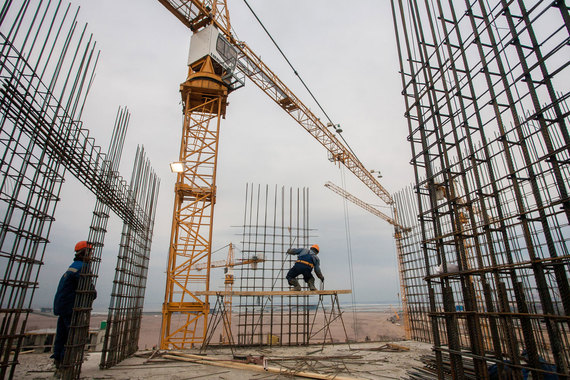
\includegraphics{images/development.jpg}
\caption{development}
\end{figure}

    \hypertarget{ux441ux43eux445ux440ux430ux43dux44fux435ux43c-ux43cux43eux434ux435ux43bux44c}{%
\section{Сохраняем
модель}\label{ux441ux43eux445ux440ux430ux43dux44fux435ux43c-ux43cux43eux434ux435ux43bux44c}}

    \begin{Verbatim}[commandchars=\\\{\}]
{\color{incolor}In [{\color{incolor} }]:} \PY{n}{joblib}\PY{o}{.}\PY{n}{dump}\PY{p}{(}\PY{n}{reg}\PY{p}{,} \PY{l+s+s1}{\PYZsq{}}\PY{l+s+s1}{model.pkl}\PY{l+s+s1}{\PYZsq{}}\PY{p}{)}
\end{Verbatim}


    \begin{figure}
\centering

\includegraphics{images/demo.png}
\caption{demo}
\end{figure}

    \hypertarget{ux441ux440ux430ux432ux43dux438ux432ux430ux435ux43c-ux441-research}{%
\section{Сравниваем с
Research}\label{ux441ux440ux430ux432ux43dux438ux432ux430ux435ux43c-ux441-research}}

    \hypertarget{iii.-production}{%
\section{III. Production}\label{iii.-production}}

\begin{figure}
\centering
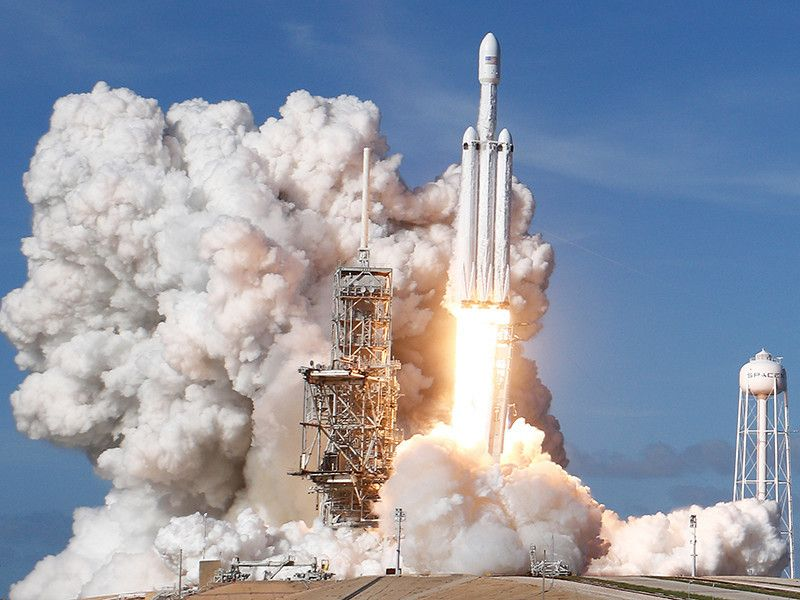
\includegraphics{images/production.jpg}
\caption{production}
\end{figure}

    \hypertarget{ux432ux43eux441ux43fux440ux43eux438ux437ux432ux43eux434ux438ux43cux43eux441ux442ux44c-ux43bux43eux433ux43eux432}{%
\section{Воспроизводимость
логов}\label{ux432ux43eux441ux43fux440ux43eux438ux437ux432ux43eux434ux438ux43cux43eux441ux442ux44c-ux43bux43eux433ux43eux432}}

\begin{figure}
\centering
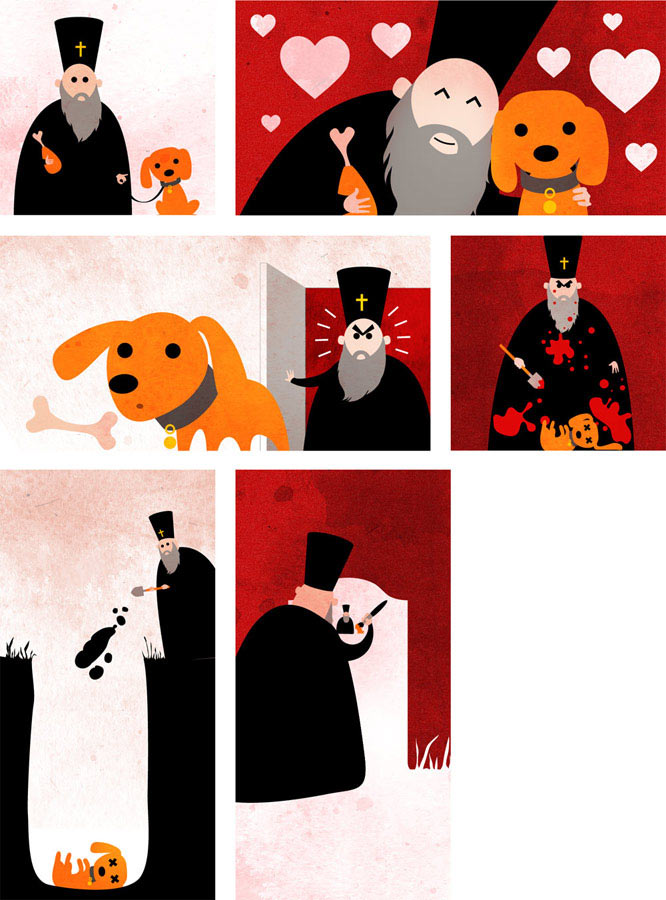
\includegraphics{images/repeat_logs.jpg}
\caption{logs}
\end{figure}

    \hypertarget{ux443ux441ux442ux430ux440ux435ux432ux430ux43dux438ux435-ux43cux43eux434ux435ux43bux438}{%
\section{Устаревание
модели}\label{ux443ux441ux442ux430ux440ux435ux432ux430ux43dux438ux435-ux43cux43eux434ux435ux43bux438}}

???

    \hypertarget{ux434ux440ux443ux433ux438ux435-ux43cux430ux442ux435ux440ux438ux430ux43bux44b}{%
\section{Другие
материалы}\label{ux434ux440ux443ux433ux438ux435-ux43cux430ux442ux435ux440ux438ux430ux43bux44b}}

\begin{itemize}
\item
\end{itemize}

    Вопросы?


    % Add a bibliography block to the postdoc
    
    
    
    \end{document}
